\documentclass{article}
\usepackage[utf8]{inputenc}
\usepackage[T1]{fontenc}
\usepackage[ngerman]{babel}
\usepackage[margin=2.5cm]{geometry}

% import math packages
\usepackage{amsmath}
\usepackage{amsfonts}
\usepackage{amssymb}
\usepackage{amsthm}
% contradiction lightning
\usepackage{stmaryrd}
% algorithms and pseudo code
\usepackage{algorithmic}
\usepackage{algorithm}
\usepackage{clrscode3e}
% formatting and layout
\usepackage{color}
% settings
\usepackage{perpage}
\MakePerPage{footnote}
% custom text colors
\definecolor{pblue}{rgb}{0.13,0.13,1}
\definecolor{pgreen}{rgb}{0,0.5,0}
% macro commands
%% requires color package and the custom colors defined here 
\newcommand{\todo}[1]{
	\addcontentsline{toc}{subsubsection}{TODO: #1}
	\textcolor{pgreen}{\texttt{\-\\ \-\\//TODO: #1\-\\ \-\\}}
}
\newcommand{\sus}[1]{
	\addcontentsline{toc}{subsection}{Übungsaufgabe #1}
	\subsection*{Übungsaufgabe #1}
	\label{ssec:#1}
}
\newcommand{\sss}[1]{
	\addcontentsline{toc}{subsubsection}{Aufgabe #1}
	\subsubsection*{Aufgabe #1}
	\label{sssec:#1}
}
\newcommand{\points}[1]{
	\begin{flushright}
		\begin{Large}
			[~~~~\string| ~#1~]
		\end{Large}
	\end{flushright}
}
% tikz
\usepackage{tikz}
\usetikzlibrary{arrows,automata,positioning}
\usepackage{pgf}

%#+-------------------------------------------------+#%
%#+						VARIABLEN			     	+#%
%#+-------------------------------------------------+#%

\begin{document}

%% Fach-Daten
\newcommand{\fachname}{Algorithmen und Datenstrukturen}
\newcommand{\stinegruppe}{Übungsgruppe 14}
%% Gruppenmitglied 1
\newcommand{\memOneName}{Utz Pöhlmann}
\newcommand{\memOneMail}{4poehlma@informatik.uni-hamburg.de}
\newcommand{\memOneNr}{6663579}
%% Gruppenmitglied 2
\newcommand{\memTwoName}{Louis Kobras}
\newcommand{\memTwoMail}{4kobras@informatik.uni-hamburg.de}
\newcommand{\memTwoNr}{6658699}
%% Gruppenmitglied 3
\newcommand{\memThreeName}{Rene Ogniwek}
\newcommand{\memThreeMail}{reneogniwek@gmx.net}
\newcommand{\memThreeNr}{6425103}
%% Gruppenmitglied 4
\newcommand{\memFourName}{Steffi Kaussow}
\newcommand{\memFourMail}{s.kaussow@gmail.com}
\newcommand{\memFourNr}{6414862}
%% Datum
\newcommand{\datum}{\today\\}






%#+-------------------------------------------------+#%
%#+						FORMATIERUNG		     	+#%
%#+-------------------------------------------------+#%

\newcommand{\fach}{
	\begin{Huge}
		\fachname\\
	\end{Huge}
}

\newcommand{\gruppe}{
	\begin{LARGE}
		\stinegruppe\\
	\end{LARGE}
}

\newcommand{\memOne}{
	\begin{center}
		\begin{Large}
			\memOneName
		\end{Large}\\
		\memOneMail\\
		\memOneNr\\
	\end{center}
	\vspace{1cm}
}
\newcommand{\memTwo}{
	\begin{center}
		\begin{Large}
			\memTwoName
		\end{Large}\\
		\memOneMail\\
		\memTwoNr\\
	\end{center}
	\vspace{1cm}
}
\newcommand{\memThree}{
	\begin{center}
		\begin{Large}
			\memThreeName
		\end{Large}\\
		\memThreeMail\\
		\memThreeNr\\
	\end{center}
	\vspace{1cm}
}
\newcommand{\memFour}{
	\begin{center}
		\begin{Large}
			\memFourName
		\end{Large}\\
		\memFourMail\\
		\memFourNr\\
	\end{center}
	\vspace{1cm}
}



%#+-------------------------------------------------+#%
%#+						DECKBLATT  			     	+#%
%#+-------------------------------------------------+#%

\thispagestyle{empty}
\-\vspace{0.5cm}
\begin{center}
	\fach
	\vspace{2cm}
	\gruppe
	\vspace{2cm}
	% group members
	\memOne
	\memTwo
	\memThree
	\memFour
	% 1 cm to next element
	\vspace{1cm}
	\datum
	\vspace{1cm}
	
	\textbf{Punkte für den Hausaufgabenteil:}\\
	\vspace{1cm}
	\begin{tabular}{c|c}
	~7.1~&~$\Sigma$~	\\	\hline
		 &
	\end{tabular}
	
\end{center}
\newpage






























%#+-------------------------------------------------+#%
%#+						INHALT  			     	+#%
%#+-------------------------------------------------+#%
\thispagestyle{empty}
\tableofcontents
\newpage


%#+-------------------------------------------------+#%
%#+						ZETTEL 1					+#%
%#+-------------------------------------------------+#%
\pagenumbering{arabic}
\section{Zettel vom 14.-16. Oktober -- Abgabe: N/A}
\subsection{Präsenzaufgabe 1.1}
%---------------%
%	Aufgabe		 %
%---------------%
Wiederholen Sie die \textit{O}-Notation und die verwandten Notationen.
Wie sind die einzelnen Mengen definiert?
Was bedeutet es, wenn $f \in O(g)$ gilt, was wenn $f \in \Theta (g)$ gilt und so weiter?\\
\vspace{1cm}
%---------------%
%	Bearbeitung	 %
%---------------%
\begin{equation*}
	\begin{array}{llll}
		O(g(n)): 		& f(n) \in O(g(n))		&\Leftrightarrow \exists c \in \mathbb{R}^+ \exists n_0 \in \mathbb{N} \forall n >= n_0 : &\|f(n)\| <= c \cdot \|g(n)\|\\
		o(g(n)): 		& f(n) \in o(g(n))		&\Leftrightarrow \forall c \in \mathbb{R}^+ \exists n_0 \in \mathbb{N} \forall n >= n_0 : &\|f(n)\| <= c \cdot \|g(n)\|\\
		\Omega(g(n)):	& f(n) \in \Omega(g(n)) &\Leftrightarrow \exists c \in \mathbb{R}^+ \exists n_0 \in \mathbb{N} \forall n >= n_0 : &\|f(n)\| >= c \cdot \|g(n)\|\\
		\omega(g(n)):	& f(n) \in \omega(g(n)) &\Leftrightarrow \forall c \in \mathbb{R}^+ \exists n_0 \in \mathbb{N} \forall n >= n_0 : &\|f(n)\| >= c \cdot \|g(n)\|\\
		\Theta(g(n)):	& f(n) \in \Theta(g(n)) &\Leftrightarrow \exists c_1, c_2 \in \mathbb{R}^+ \exists n_0 \in \mathbb{N} \forall n >= n_0 : &c_1 \cdot \|g(n)\| <= \|f(n)\| <= c_2 \cdot \|g(n)\|
	\end{array}
\end{equation*}
\subsection{Präsenzaufgabe 1.2}
%---------------%
%	Aufgabe	 	 %
%---------------%
Beweisen Sie:
\begin{itemize}
	\item $n^2+3n-5 \in O(n^2)$
	\item $n^2-2n \in \Theta(n^2)$
	\item $n! \in O((n+1)!)$
\end{itemize}
Gilt im letzten Fall auch $n! \in o((n+1)!)$?\\
\vspace{1cm}
%---------------%
%	Bearbeitung	%
%---------------%
\begin{equation*}
\begin{array}{rl}
	f(n) \in O(g(n)) &\Leftrightarrow lim_{n\rightarrow \infty} \frac{f(n)}{g(n)} < \infty\\
	f(n) &= n^2+3n-5\\
	g(n) &= n^2\\
	\frac{f(n)}{g(n)} &= \frac{n^2+3n-5}{n^2}
	\vspace{0.5cm}\\
	lim_{n \rightarrow \infty} \frac{n^2+3n-5}{n^2} &= lim_{n \rightarrow \infty} 1+\frac{3}{n}-\frac{5}{n^2}\\
		&=1+\frac{3}{\infty}-\frac{5}{\infty^2}\\
		&=1+0+0\\
		&=1 < \infty \Rightarrow f(n) \in O(g(n))
\end{array}
\end{equation*}
\begin{flushright}
$\square$
\end{flushright}
\vspace{1cm}
\begin{equation*}
\begin{array}{rl}
	c_1, c_2 \in \mathbb{R}^+,n_0 \in \mathbb{N} \forall n >= n_0:	& c_1 \cdot n^2<= n^2-2n <= c_2 \cdot n^2\\
		\Leftrightarrow & c_1 <= 1-\frac{1}{n} <= c_2
\end{array}
\end{equation*}
Dies ist erfüllbar ab $n_0 >= 2$ , da für $n=1$ im mittleren Ausdruck 0 herauskommt und $c_1$ größer als 0, aber kleiner als der mittlere Ausdruck sein muss.
Ist $n >= 2$, so kommt im mittleren Ausdruck $0,5$ heraus, für $c_1$ lässt sich ein beliebiger Wert aus $\string]0;0.5\string[$ wählen, sei es an dieser Stelle $\frac{1}{4}$.
Als Obergrenze für $c_2$ lässt sich jeder Wert größer oder gleich 1 wählen, da der mittlere Ausdruck nicht größer als 1 werden kann und somit die Bedingung des "kleiner gleich" sofort erfüllt ist.\\
Somit wird als Ergebnis für die Belegung gewählt: $c_1 = \frac{1}{4}; c_2 = 1; n_0 = 2$.
Mit dieser Belegung gilt $n^2-2n \in \Theta(n^2)$
\begin{flushright}
$\square$
\end{flushright}
\vspace{1cm}
\begin{equation*}
\begin{array}{rl}
	f(n) \in O(g(n)) &\Leftrightarrow lim_{n\rightarrow \infty} \frac{f(n)}{g(n)} < \infty\\
	f(n) &= n!\\
	g(n) &= (n+1)! = (n+1) \cdot n!
	\vspace{0.5cm}\\
	lim_{n\rightarrow \infty} \frac{n!}{(n+1) \cdot n!} &= lim_{n \rightarrow \infty} \frac{1}{n+1}\\
		&= \frac{1}{\infty}\\
		&= 0 < \infty \Rightarrow f(n) \in O(g(n))
\end{array}
\end{equation*}
Da die Bedingung für $o(g(n))$ ist, dass der Quotient nicht nur kleiner unendlich, sondern gleich null ist, was hier wie oben gezeigt gegeben ist, gilt auch $n! \in o((n+1)!)$.
\begin{flushright}
$\square$
\end{flushright}
\subsection{Präsenzaufgabe 1.3}
%---------------%
%	Aufgabe		%
%---------------%
Beweisen oder widerlegen Sie:
\begin{enumerate}
	\item $ f(n),g(n) \in O(h(n)) \Rightarrow f(n)+g(n) \in O(h(n)) $
	\item $ f(n),g(n) \in O(h(n)) \Rightarrow f(n) \cdot g(n) \in O(h(n)) $
\end{enumerate}
\vspace{1cm}
%---------------%
%	Bearbeitung	%
%---------------%
\[
	\exists c_1 \in \mathbb{R}^+ \exists n_{0_1} \in \mathbb{N} \forall n >= n_{0_1} : \|f(n)\| <= c_1 \cdot \|h(n)\|
\]
\[
	\exists c21 \in \mathbb{R}^+ \exists n_{0_2} \in \mathbb{N} \forall n >= n_{0_2} : \|g(n)\| <= c_2 \cdot \|h(n)\|
\]
\[
	n_0 = max(n_{0_1},n_{0_2})
\]
\[
	\|f(n)+g(n)\| <= c_1\cdot\|h(n)\|+c_2\cdot\|h(n)\| <= (c_1+c_2)\cdot\|h(n)\|
\]
\vspace{0.5cm}\\
Seien $f(n)$ und $g(n)$ Polynome zweiten Grades sowie $h(n)$ ein Polynom dritten Grades.
Dann sind sowohl $f(n)$ als auch $g(n)$ durch die \textit{limes}-Bedingung in $O(h(n))$.
Das Produkt zweier Polynome zweiten Grades ist allerdings ein Polynom vierten Grades, sodass gilt:
\begin{equation*}
	\lim_{n\rightarrow\infty}\frac{n^2 \cdot n^2}{n^3}=\lim_{n\rightarrow\infty}\frac{n^4}{n^3}=\lim_{n\rightarrow\infty}n=\infty
\end{equation*}
Damit ist das Produkt der Polynome nicht mehr in $O(h(n))$, da die \textit{limes}-Bedingung, nach der der Quotient der Polynome für \textit{n} gegen Unendlich kleiner als Unendlich sein zu hat, nicht erfüllt ist.
Damit ist (2) widerlegt.
\begin{flushright}
$\square$
\end{flushright}
\newpage
%#+-------------------------------------------------+#%
%#+						ZETTEL 2					+#%
%#+-------------------------------------------------+#%
\section{Zettel vom 15.10. -- Abgabe: 26.10.}
\subsection{Übungsaufgabe 2.1}
\begin{flushright}
\begin{Large}
[~~~~\string| ~~2~]
\end{Large}
\end{flushright}
%---------------%
%	Aufgabe		%
%---------------%
Begründen Sie formal, warum folgende Größenabschätzungen gelten bzw. nicht gelten:
\begin{enumerate}
	\item $3n^3-6n+20 \in O(n^3)$
	\item $n^2 \cdot \operatorname{log} n \in O(n^3) \cap \Omega(n^2)$
\end{enumerate}
\vspace{1cm}
%---------------%
%	Bearbeitung	%
%---------------%
\subsubsection{}
\[
	3n^3-6n+20 \in O(n^3) \Leftrightarrow lim_{n\rightarrow\infty}\frac{3n^3-6n+20}{n^3} < \infty
\]
\[
	lim_{n\rightarrow\infty}\frac{3n^3-6n+20}{n^3} = lim_{n\rightarrow\infty} \frac{3n^3}{n^3}-\frac{6n}{n^3}+\frac{20}{n^3}=lim_{n\rightarrow\infty}3-\frac{6}{n^2}+\frac{20}{n^3}=3-0+0<\infty
\]
\[
	\Rightarrow 3n^3-6n+20 \in O(n^3)  ~~~~~~~~\square
\]
\subsubsection{}
\[
	n^2 \cdot \operatorname{log} n \in O(n^3) \cap \Omega(n^2) \Leftrightarrow lim_{n\rightarrow\infty} \frac{n^2 \cdot \operatorname{log} n}{n^3} < \infty \land lim_{n\rightarrow\infty} \frac{n^2 \cdot \operatorname{log} n}{n^2} > 0
\]
\[
	\frac{n^2 \cdot \operatorname{log} n}{n^2} = \frac{1 \cdot \operatorname{log} n}{1} = \operatorname{log} n > 0~ \forall n > 1 \Rightarrow n^2 \cdot \operatorname{log} n \in \Omega(n^2)
\]
\[
	lim_{n\rightarrow\infty} \frac{n^2 \cdot \operatorname{log} n}{n^3} = lim_{n\rightarrow\infty} \frac{\operatorname{log} n}{n} \overset{\text{l'H}}{=} lim_{n\rightarrow\infty}\frac{1}{n} \cdot \frac{1}{1} = lim_{n\rightarrow\infty} \frac{1}{n} = \frac{1}{\infty} = 0 \Rightarrow n^2\cdot\operatorname{log} n \in  O(n^3)
\]
\[
	\Rightarrow n^2 \cdot \operatorname{log} n \in O(n^3) \cap \Omega(n^2)~~~~\square
\]
\subsection{Übungsaufgabe 2.2}
\begin{flushright}
\begin{Large}
[~~~~\string| ~~4~]
\end{Large}
\end{flushright}
%---------------%
%	Aufgabe		%
%---------------%
Ordnen Sie die folgenden Funktionen nach ihrem Wachstumsgrad in aufsteigender Reihenfolge, d.h. folgt eine Funktion $g(n)$ einer Funktion $f(n)$, so soll $f(n) \in O(g(n))$ gelten.
\[
	n, \operatorname{log} n, n^2, n^{\frac{1}{2}}, \sqrt{n}^3, 2^n, \operatorname{ln} n, 1000
\]
Mit log ist hier der Logarithmus zur Basis 2, mit ln der natürliche Logarithmus (Basis \textit{e}) gemeint.
Begründen Sie stets Ihre Aussage.
Zwei Funktionen $f(n)$ und $g(n)$ befinden sich ferner in der selben Äquivalenzklasse, wenn $f(n) \in \Theta (g(n))$ gilt.
Geben Sie an, welche Funktionen sich in derselben Äquivalenzklasse befinden und begründen Sie auch hier ihre Aussage.\\
\vspace{1cm}\\
%---------------%
%	Bearbeitung	%
%---------------%
Die bearbeitete Menge wird i.F. als $M_F$ bezeichnet.
Die Menge, die gerade alle Elemente von $M_F$ in aufsteigend sortierter Reihenfolge enthält, wird als $M_F'$ bezeichnet.\\
$M_F$ wird mit \textsc{InsertionSort} in $M_F'$ hineinsortiert.\\ \vspace{0.5cm}
Sei $e \in M_F$.
Für $e$ wird das Element $1000$ gewählt.
Da $\string|M_F'\string|$ leer ist, muss $1000$ nicht weiter geprüft werden.
\begin{flushright}
	$M_F' = \{1000\}$
\end{flushright}
$e$ wird nun über $M_F$ iteriert, bis $M_F' = Sorted(M_F)$. \vspace{0.5cm}\\
$e = n$
\begin{equation*}
	\begin{array}{lllll}
		f(n) = n\\
		g(n) = 1000	&	\underset{n\rightarrow\infty}{lim}	\frac{n}{1000}	&=	\infty	&\Rightarrow n \not \in O(1000)
		\\\\
		f(n) = 1000\\
		g(n) = n & \underset{n\rightarrow\infty}{lim} \frac{1000}{n} &= 0 &\Rightarrow 1000 \in O(n) &\Rightarrow  n \text{ folgt } 1000
	\end{array}
\end{equation*}
\begin{flushright}
	$M_F' = \{1000,n\}$
\end{flushright}
\vspace{0.6cm}
$e = \operatorname{log} n$
\begin{equation*}
	\begin{array}{lllll}
		f(n) = log(n)\\
		g(n) = n & \underset{n\rightarrow\infty}{lim} \frac{log(n)}{n} \overset{\text{L'Hospital}}{=} \underset{n\rightarrow\infty}{lim} \frac{\frac{1}{ln(2) \cdot n}}{1} = \underset{n\rightarrow\infty}{lim}\frac{1}{ln(2) \cdot n} &= 0 &\Rightarrow log(n) \in O(n) &\Rightarrow  n \text{ folgt } log(n)
		\\\\
		f(n) = log(n)\\
		g(n) = 1000 & \underset{n\rightarrow\infty}{lim} \frac{log(n)}{1000} &= \infty &\Rightarrow log(n) \not \in O(1000)
	\end{array}
\end{equation*}
\begin{flushright}
	$M_F' = \{1000,\operatorname{log}n,n\}$
\end{flushright}
\vspace{0.6cm}
$e = 4$
\begin{equation*}
	\begin{array}{lllll}
		f(n) = 4\\
		g(n) = n & \underset{n\rightarrow\infty}{lim} \frac{4}{n} &= 0 &\Rightarrow 4 \in O(n) &\Rightarrow  n \text{ folgt } 4
		\\\\
		f(n) = 4\\
		g(n) = log(n) & \underset{n\rightarrow\infty}{lim} \frac{4}{log(n)} &= 0 &\Rightarrow 4 \in O(log(n)) &\Rightarrow  log(n) \text{ folgt } 4
		\\\\
		f(n) = 4\\
		g(n) = 1000 & \underset{n\rightarrow\infty}{lim} \frac{4}{1000} &= 0,004 &\Rightarrow 4 \in \Theta(1000) &\Rightarrow  4 \text{ und } 1000 \text{ befinden sich in der selben Ä.-klasse}
	\end{array}
\end{equation*}
\begin{flushright}
	$M_F' = \{4,1000,\operatorname{log}n,n\}$
\end{flushright}
\vspace{0.6cm}
$e = n^2$
\begin{equation*}
	\begin{array}{lllll}
		f(n) = n^2\\
		g(n) = n	&	\underset{n\rightarrow\infty}{lim}	\frac{n^2}{n}	&=	\infty	&\Rightarrow n^2 \not \in O(n)
		\\\\
		f(n) = n\\
		g(n) = n^2 & \underset{n\rightarrow\infty}{lim} \frac{n}{n^2} &= 0 &\Rightarrow n \in O(n^2) &\Rightarrow  n^2 \text{ folgt } n
	\end{array}
\end{equation*}
\begin{flushright}
	$M_F' = \{4,1000,\operatorname{log}n,n,n^2\}$
\end{flushright}
\vspace{0.6cm}
$e = n^{\frac{1}{2}}$
\begin{equation*}
	\begin{array}{lllll}
		f(n) = n^\frac{1}{2}\\
		g(n) = n^2	&	\underset{n\rightarrow\infty}{lim}	\frac{n^\frac{1}{2}}{n^2} = \underset{n\rightarrow\infty}{lim} \frac{1}{n^\frac{3}{2}} &=	0	&\Rightarrow n^\frac{1}{2} \in O(n^2) &\Rightarrow n^2 \text{ folgt } n^\frac{1}{2}
		\\\\
		f(n) = n^\frac{1}{2}\\
		g(n) = n & \underset{n\rightarrow\infty}{lim} \frac{n^\frac{1}{2}}{n} = \underset{n\rightarrow\infty}{lim} \frac{1}{n^\frac{1}{2}} &= 0 &\Rightarrow n^\frac{1}{2} \in O(n) &\Rightarrow  n \text{ folgt } n^\frac{1}{2}
		\\\\
		f(n) = n^\frac{1}{2}\\
		g(n) = log(n) & \underset{n\rightarrow\infty}{lim} \frac{n^\frac{1}{2}}{log(n)} \overset{\text{L'Hospital}}{=} \underset{n\rightarrow\infty}{lim} \frac{\frac{1}{2}\cdot n^{-\frac{1}{2}}}{\frac{1}{ln(2)\cdot n}} = \underset{n\rightarrow\infty}{lim} \frac{ln(2)\cdot n^\frac{1}{2}}{2} &= \infty &\Rightarrow n^\frac{1}{2} \not \in O(log(n))
	\end{array}
\end{equation*}
\begin{flushright}
	$M_F' = \{4,1000,\operatorname{log}n,n^\frac{1}{2},n,n^2\}$
\end{flushright}
\vspace{0.6cm}
$e = \sqrt{n}^3$
\begin{equation*}
	\begin{array}{lllll}
		f(n) = \sqrt{n}^3\\
		g(n) = n^2	&	\underset{n\rightarrow\infty}{lim}	\frac{\sqrt{n}^3}{n^2}	= \underset{n\rightarrow\infty}{lim} \frac{1}{n^\frac{1}{2}} &=	0	&\Rightarrow \sqrt{n}^3 \in O(n^2) &\Rightarrow n^2 \text{ folgt } \sqrt{n}^3
		\\\\
		f(n) = \sqrt{n}^3\\
		g(n) = n & \underset{n\rightarrow\infty}{lim} \frac{\sqrt{n}^3}{n} = \underset{n\rightarrow\infty}{lim} n^\frac{1}{2} &= \infty &\Rightarrow \sqrt{n}^3 \not \in O(n)
	\end{array}
\end{equation*}
\begin{flushright}
	$M_F' = \{4,1000,\operatorname{log}n,n^\frac{1}{2},n,\sqrt{n}^3,n^2\}$
\end{flushright}
\vspace{0.6cm}
$e = 2^n$
\begin{equation*}
	\begin{array}{lllll}
		f(n) = 2^n\\
		g(n) = n^2	&	\underset{n\rightarrow\infty}{lim}	\frac{2^n}{n^2}	\overset{\text{L'Hospital}}{=} \underset{n\rightarrow\infty}{lim} \frac{ln(2)\cdot 2^n}{2 \cdot n} \overset{\text{L'Hospital}}{=} \underset{n\rightarrow\infty}{lim} \frac{ln^2(2)\cdot 2^n}{2} &=	\infty	&\Rightarrow 2^n \not \in O(n^2)
		\\\\
		f(n) = n^2\\
		g(n) = 2^n & \underset{n\rightarrow\infty}{lim} \frac{n^2}{2^n} \overset{\text{L'Hospital}}{=} \underset{n\rightarrow\infty}{lim} \frac{2 \cdot n}{ln(2)\cdot 2^n} \overset{\text{L'Hospital}}{=} \underset{n\rightarrow\infty}{lim} \frac{2}{ln^2(2)\cdot 2^n} &= 0 &\Rightarrow n^2 \in O(2^n) &\Rightarrow  n^2 \text{ folgt } 2^n
	\end{array}
\end{equation*}
\begin{flushright}
	$M_F' = \{4,1000,\operatorname{log}n,n^{\frac{1}{2}},n,\sqrt{n}^3,n^2,2^n\}$
\end{flushright}
\vspace{0.6cm}
$e = \operatorname{ln}n$
\begin{equation*}
	\begin{array}{lllll}
		f(n) = ln(n)\\
		g(n) = 2^n & \underset{n\rightarrow\infty}{lim} \frac{ln(n)}{2^n} \overset{\text{L'Hospital}}{=} \underset{n\rightarrow\infty}{lim} \frac{\frac{1}{n}}{ln(2)\cdot 2^n} = \underset{n\rightarrow\infty}{lim}\frac{1}{n\cdot ln(n) \cdot 2^n} &= 0 &\Rightarrow ln(n) \in O(2^n) &\Rightarrow  2^n \text{ folgt } ln(n)
		\\\\
		f(n) = ln(n)\\
		g(n) = n^2 & \underset{n\rightarrow\infty}{lim} \frac{ln(n)}{n^2} \overset{\text{L'Hospital}}{=} \underset{n\rightarrow\infty}{lim} \frac{\frac{1}{n}}{2\cdot n} = \underset{n\rightarrow\infty}{lim}\frac{1}{2\cdot n^2} &= 0 &\Rightarrow ln(n) \in O(n^2) &\Rightarrow  n^2 \text{ folgt } ln(n)
		\\\\
		f(n) = ln(n)\\
		g(n) = \sqrt{n}^3 & \underset{n\rightarrow\infty}{lim} \frac{ln(n)}{\sqrt{n}^3} \overset{\text{L'Hospital}}{=} \underset{n\rightarrow\infty}{lim}\frac{\sqrt[3]{n}}{2\cdot n} \overset{\text{L'Hospital}}{=} \underset{n\rightarrow\infty}{lim} \frac{1}{6\cdot n^\frac{2}{3}} &= 0 &\Rightarrow ln(n) \in O(\sqrt{n}^3) &\Rightarrow  \sqrt{n}^3 \text{ folgt } ln(n)
		\\\\
		f(n) = ln(n)\\
		g(n) = n & \underset{n\rightarrow\infty}{lim} \frac{ln(n)}{n} \overset{\text{L'Hospital}}{=} \underset{n\rightarrow\infty}{lim} \frac{\frac{1}{n}}{1} = \underset{n\rightarrow\infty}{lim}\frac{1}{n} &= 0 &\Rightarrow ln(n) \in O(n) &\Rightarrow  n \text{ folgt } ln(n)
		\\\\
		f(n) = ln(n)\\
		g(n) = n^\frac{1}{2} & \underset{n\rightarrow\infty}{lim} \frac{ln(n)}{n^\frac{1}{2}} \overset{\text{L'Hospital}}{=} \underset{n\rightarrow\infty}{lim} \frac{\frac{1}{n}}{\frac{1}{2\cdot n^\frac{1}{2}}} = \underset{n\rightarrow\infty}{lim}\frac{2}{n^\frac{1}{2}} &= 0 &\Rightarrow ln(n) \in O(n^\frac{1}{2}) &\Rightarrow  n^\frac{1}{2} \text{ folgt } ln(n)
		\\\\
		f(n) = ln(n)\\
		g(n) = log(n) & \underset{n\rightarrow\infty}{lim} \frac{ln(n)}{log(n)} \overset{\text{L'Hospital}}{=} \underset{n\rightarrow\infty}{lim} \frac{\frac{1}{n}}{\frac{1}{ln(2) \cdot n}} &= ln(2) &\Rightarrow ln(n) \in \Theta(log(n)) &\Rightarrow  ln(n) \text{ und } log(n)\\ &&&\text{ befinden sich in der}&\text{selben Ä.-klasse}
	\end{array}
\end{equation*}
\begin{flushright}
	$M_F' = \{4,1000,\operatorname{ln} n, \operatorname{log} n, n^{\frac{1}{2}}, n, \sqrt{n}^3, n^2, 2^n\}$
\end{flushright}
In der selben Äquivalenzklasse befinden sich zum einen $4$ und $1000$ und zum anderen $log(n)$ und $ln(n)$. Die restlichen Werte sind jeweils alleine in ihrer Äquivalenzklasse.
\\
\subsection{Übungsaufgabe 2.3}
\begin{flushright}
\begin{Large}
[~~~~\string| ~~2~]
\end{Large}
\end{flushright}
%---------------%
%	Aufgabe		%
%---------------%
Beweisen oder widerlegen Sie:
\[
	f(n),g(n) \in O(h(n)) \Rightarrow f(n)\cdot g(n) \in O((h(n))^2)
\]
\vspace{1cm}\\
%---------------%
%	Bearbeitung	%
%---------------%
Für diesen Beweis wird der Beweis des dritten Satzes der Summen- und Produkteigenschaften der O-Notation\footnote{vgl. Vorlesung, Foliensatz 1 (14.10.), S.33} zu Hilfe genommen:
\begin{proof}
Sei $f\in O(h_1)$ und $g\in O(h_2)$, dann gibt es ein $c$, $n_0$, so dass $f(n) \leq c \cdot h_1(n) \forall n \geq n_0$ und ebenso $c', n_0'$, so dass $g(n') \leq c' \cdot h_2(n') \forall n' \geq n_0'$.
Daraus folgt $f(n'')\cdot g(n'') \leq c \cdot c' \cdot h_1(n'') \cdot h_2(n'') \forall n'' \geq max(n_0, n_0')$, also $f \cdot g \in O(h_1 \cdot h_2)$.
\end{proof}
Setzt man nun $h_1, h_2 = h$ folgt daraus für den letzten Ausdruck des Beweises $f(n) \cdot g(n) \in O(h(n) \cdot h(n)) \Rightarrow f(n) \cdot g(n) \in O((h(n))^2)$.

\subsection{Übungsaufgabe 2.4}
\begin{flushright}
\begin{Large}
[~~~~\string| ~~8~]
\end{Large}
\end{flushright}
%---------------%
%	Aufgabe		%
%---------------%
Seien
\begin{enumerate}
	\item 
	\[
		T(n) :=  \begin{cases}
					\begin{array}{ll}
						0, & \text{für }n=0\\
						3 \cdot T(n-1)+2, &\text{sonst}
					\end{array}
				\end{cases}
	\]
	\item
	\[
		S(n) := \begin{cases}
					\begin{array}{ll}
						c,			& \text{für }n=1\\
						16 \cdot S(\frac{n}{4})+n^2, & \text{sonst}
					\end{array}
				\end{cases}
	\]
\end{enumerate}
Rekurrenzgleichungen (\textit{c} ist dabei eine Konstante).
\vspace{0.2cm}\\
Bestimmen Sie wie in der Vorlesung jeweils die Größenordnung der Funktion $T: \mathbb{N} \rightarrow \mathbb{N}$ einmals mittels der (a) Substitutionsmethode und einmal mittes des (b) Mastertheorems.
Ihre Ergebnisse sollten zumindest hinsichtlich der O-Notation gleich sein, so dass Sie etwaige Rechenfehler entdecken können!
Führen Sie bei (a) auch den Induktionsbeweis, der in der Vorlesung übersprungen wurde!
\vspace{1cm}\\
%---------------%
%	Bearbeitung	%
%---------------%
\subsubsection{2.4.1}
    \begin{enumerate}
        \item [a)]
        \[
            \begin{array}{lll}
                T(n)~&=~3 \cdot T(n-1)+2 &\\
                &=~3*(3*T(n-2)+2)+2~&=~3^2*T(n-2)+3^2-1\\
                &=~3^2*(3*T(n-3)+2)+8~&=~3^3*T(n-3)+3^3-1\\
                &=~...&\\
                &=~3^k*T(n-k)+3^k-1
            \end{array}
        \]
        \\
        Wir kommen auf eine sinnvolle Verallgemeinerung der Formel.\\
        Beweis der Formel durch vollständige Induktion:\\\\
        Induktionsanfang: $T(0)$ gilt nach Definiton.\\
        Induktionsschritt: Sei $n \in \mathbb{N}$ (s. Aufgabenstellung). Wir nehmen an, dass $T(n)$ gilt (Induktionsannahme) und zeigen $T(n+1)$. Es gilt\\
        \[
            \begin{array}{ll}
                T(n)~&=~3*T(n-1)+2\\
                T(n+1)~&=~3*T(n+1-1)+2\\
                &=~3*T(n)+2
                \\\\
                T(n)~&=~3^k*T(n-k)+3^k-1\\
                T(n+1)~&=~3^k*T(n+1-k)+3^k-1
            \end{array}
        \]
        Das zeigt $T(n+1)$.\\
        Damit sind der Induktionsanfang und der Induktionsschritt bewiesen. Es folgt, dass $T(n)$ für alle $n \in \mathbb{N}$ gilt.\\
        \\
        Da die Rekursion bei $T(0)~=~0$, also $n-k~=~0$ abbricht, wird mit $k~=~n$ weiter gerechnet.\\
        \[
            \begin{array}{ll}
                T(n)~&=~3^k*T(n-k)+3^k-1\\
                &=~3^n*T(n-n)+3^n-1\\
                &=~3^n*T(0)+3^n-1\\
                &=~3^n*0+3^n-1\\
                &=~3^n-1 \in \Theta (3^n)
            \end{array}
        \]
        \item [b)]
        Das Mastertheorem ist auf Aufgabe 1. nicht anwendbar, da die Form\\
        \[
		T(n) :=  \begin{cases}
					\begin{array}{ll}
						c, & \text{falls }n=1\\
						a \cdot T(\frac{n}{b})+f(n), &\text{falls }n>1
					\end{array}
				\end{cases}
    	\]
    	\\
    	bei\\
    	\[
		T(n) :=  \begin{cases}
					\begin{array}{ll}
						0, & \text{für }n=0\\
						3 \cdot T(n-1)+2, &\text{sonst}
					\end{array}
				\end{cases}
    	\]
    	\\
    	nicht eingehalten wurde.
    \end{enumerate}
\subsubsection{2.4.2}
    \begin{enumerate}
        \item [a)]
        \[
            \begin{array}{ll}
                S(n)~&=~16 \cdot S(\frac{n}{4})+n^2\\
                &=~16 \cdot S(\frac{16 \cdot S(\frac{n}{4})+n^2}{4})+n^2\\
                &=~16 \cdot S(\frac{16 \cdot S(\frac{16 \cdot S(\frac{n}{4})+n^2}{4})+n^2}{4})+n^2\\
                &=~16 \cdot S(\frac{16 \cdot S(\frac{16 \cdot S(\frac{16 \cdot S(\frac{n}{4})+n^2}{4})+n^2}{4})+n^2}{4})+n^2\\
                &=~16 \cdot S(\frac{16 \cdot S(\frac{16 \cdot S(\frac{16 \cdot S(\frac{16 \cdot S(\frac{n}{4})+n^2}{4})+n^2}{4})+n^2}{4})+n^2}{4})+n^2
            \end{array}
        \]
        \\
        Keine sinnvolle Vereinfachung erkennbar. $=>$ Substitutionsmethode nicht anwendbar.
        \item [b)]
        Die Form\\
        \[
		S(n) :=  \begin{cases}
					\begin{array}{ll}
						c, & \text{falls }n=1\\
						a \cdot T(\frac{n}{b})+f(n), &\text{falls }n>1
					\end{array}
				\end{cases}
    	\]
    	\\
    	ist bei\\
    	\[
		S(n) := \begin{cases}
					\begin{array}{ll}
						c,			& \text{für }n=1\\
						16 \cdot S(\frac{n}{4})+n^2, & \text{sonst}
					\end{array}
				\end{cases}
    	\]
    	\\
    	eingehalten. Das Mastertheorem ist daher anwendbar.\\
    	\\
    	\begin{enumerate}
    	    \item[I.]
    	    $S(n) \in \Theta (n^{log_b(a)})$, falls $f(n) \in O(n^{log_b(a)- \epsilon})$ für ein $\epsilon > 0$.\\
    	    \\
    	    \[
    	        \begin{array}{ll}
    	            f(n) &\in O(n^{log_b(a)- \epsilon})\\
    	            n^2 &\in O(n^{log_4(16)- \epsilon})\\
    	            n^2 &\in O(n^{2- \epsilon})
    	        \end{array}
    	    \]
    	    \\
    	    Hierfür kann kein $\epsilon$ gefunden werden. Daher gilt diese Aussage nicht\\
    	    \item[II.]
    	    $S(n) \in \Theta (n^{log_b(a)} \cdot log_2(n))$, falls $f(n) \in \Theta (n^{log_b(a)})$.\\
    	    \[
    	        \begin{array}{ll}
    	            f(n) &\in O(n^{log_b(a)})\\
    	            n^2 &\in O(n^{log_4(16)})\\
    	            n^2 &\in O(n^2)
    	        \end{array}
    	    \]
    	    \\
    	    Dies stimmt, daher gilt diese Aussage.
    	    \item[III.]
    	    $S(n) \in \Theta (f(n))$, falls $f(n) \in \Omega (n^{log_b(a)+ \epsilon})$ für ein $\epsilon > 0$ \textbf{und} $a \cdot f(\frac{n}{b}) \leq \delta \cdot f(n)$ für ein $\delta < 1$ und große $n$.\\
    	    \\
    	    \[
    	        \begin{array}{ll}
    	            f(n) &\in \Omega (n^{log_b(a)+ \epsilon})\\
    	            n^2 &\in \Omega (n^{log_4(16)+ \epsilon})\\
    	            n^2 &\in \Omega (n^{2+ \epsilon})
    	        \end{array}
    	    \]
    	    \\
    	    Dies stimmt für alle $\epsilon \geq 0$, also auch für mindestens ein $\epsilon > 0$.
    	    \[
    	        \begin{array}{lll}
    	            a \cdot f(\frac{n}{b}) \leq \delta \cdot f(n)~~~~~~~~~~~~~~~~~~~~~~~&\text{\textbackslash einsetzen}\\
    	            16 \cdot (\frac{n}{4})^2 \leq \delta \cdot n^2 &\text{\textbackslash $\sqrt()$}\\
    	            4 \cdot \frac{n}{4} \leq \sqrt{\delta} \cdot n\\
    	            n \leq \sqrt{\delta} \cdot n &\text{\textbackslash :n    (n ist immer positiv, da $n \in \mathbb{N}$, s. Aufgabenstellung)}\\
    	            1 \leq \sqrt{\delta} &\text{\textbackslash $()^2$}\\
    	            1 \leq \delta
    	        \end{array}
    	    \]
    	    \\
    	    Damit ist $\delta \geq 1$ und nicht, wie benötigt, $\delta < 1$. Daher gilt diese Aussage nicht.
    	    \\\\
    	    Da nur II. gilt, gilt $S(n) \in \Theta (n^{log_b(a)} \cdot log_2(n))$, also $S(n) \in \Theta (n^2 \cdot log_2(n))$.
    	\end{enumerate}
    \end{enumerate}
\newpage
%#+-------------------------------------------------+#%
%#+						ZETTEL 3					+#%
%#+-------------------------------------------------+#%
\section{Zettel vom 29. 10. -- Abgabe: 09. 11.}
\subsection{Übungsaufgabe 3.1}
\begin{flushright}
\begin{Large}
[~~~~\string| ~~3~]
\end{Large}
\end{flushright}
%---------------%
%	Aufgabe		%
%---------------%
Gegeben seien die folgenden Code-Fragmente.
Geben Sie eine möglichst dichte asymptotische obere Schranke für die Laufzeit der einzelnen Code-Fragmente jeweils in Abhängigkeit von $n$ an.
Begründen Sie Ihre Behauptung.
(Es geht hier nicht um die Bedeutung des Codes, nur um die Laufzeit.
An der Stelle von $sum = sum + j$ könnte sinnvoller(er) Code stehen.
Die Einrückung gibt den Skopus der Schleifenkonstrukte an.) \\
\vspace{0.3cm}
\begin{minipage}[t]{0.32\textwidth}
	\begin{codebox}
		\Procname{\textsc{Algo1()}}
		\li \For $i \gets 0$ \To $n$
		\Indentmore
			\li \For $j \gets n$ \Downto $1$
			\Indentmore
				\li $sum \gets sum+j$
			\End
			\li \For $j \gets 1$ \To $n$
			\Indentmore
				\li $sum \gets sum+j$
			\End
		\End
	\end{codebox}
\end{minipage}
\begin{minipage}[t]{0.32\textwidth}
	\begin{codebox}
		\Procname{\textsc{Algo2()}}
		\li $i \gets 1$
		\li \While $i < 2 \cdot n$
		\Indentmore
			\li \For $j \gets 1$ \To $i$
			\Indentmore
				\li $sum \gets sum+j$
			\End
			\li $i \gets i+2$
		\End
	\end{codebox}
\end{minipage}
\begin{minipage}[t]{0.32\textwidth}
	\begin{codebox}
		\Procname{\textsc{Algo3()}}
		\li $i \gets 1$
		\li \While $i \cdot i < n$
		\Indentmore
			\li $i \gets i+1$
			\li $j \gets n$
			\li \While $j > 1$
			\Indentmore
				\li $sum \gets sum+j$
				\li $j \gets j/2$
			\End
		\End
	\end{codebox}
\end{minipage}
\vspace{1cm}\-\\
%---------------%
%	Bearbeitung	%
%---------------%
\subsubsection{Aufgabe 3.1.1}
Der Algorithmus läuft in $O(n^2)$.\\
Bei beiden inneren \textbf{for}-Blöcke laufen jeweils $n-1$ mal durch, sodass der innere Block insgesamt $2 \cdot (n-1)=2n-2$ mal ausgeführt wird.
Die äußere \textbf{for}-Schleife läuft gerade $n$ mal; also wird der Block der Länge $2n-2$ $n$ mal ausgeführt.
Dies führt zu einer Laufzeit von $n \cdot (2n-2)=2n^2-2n \in \mathcal{O}(n^2)$.
\subsubsection{Aufgabe 3.1.2}
Die äußere Schleife läuft zwar bis $2\cdot n$, da die Zählvariable allerdings in Zweierschritten inkrementiert wird, wird die Schleife $n$ mal durchlaufen.
Die innere Schleife wird $n\cdot(n-1)$ mal durchlaufen ($1+3+5+7+\dots+2\cdot n-3+2\cdot n-1=n\cdot(n-1)$.
Dies ergibt insgesamt eine Laufzeit von $n \cdot n \cdot (n-1) = n^3-n^2 \in \mathcal{O}(n^3)$
\subsubsection{Aufgabe 3.1.3}
Die äußere Schleife wird $\sqrt{n}$ mal durchlaufen, da $i^2=n\Rightarrow i=\sqrt{n}$.
Zeilen 5-7 laufen in $\operatorname{log} n$.
Das ergibt eine Gesamtlaufzeit in $\mathcal{O}(\sqrt{n}\cdot\operatorname{log} n)$
\subsection{Übungsaufgabe 3.2}
\begin{flushright}
\begin{Large}
[~~~~\string| ~~2~]
\end{Large}
\end{flushright}
%---------------%
%	Aufgabe		%
%---------------%
Gegeben sei folgender Algorithmus, der ein Array \textit{A} als Eingabe erwartet (dessen genaue Funktionsweise nachfolgend aber nicht wichtig ist):\\
\begin{algorithm}[H]
\caption{FUNC(A)}
\begin{algorithmic}[1]
\IF{$A.länge < 4$}
	\RETURN $4$
\ELSE
	\STATE $sum = 0$
	\FOR{$i=1$ to $A.laenge$}
		\STATE $sum = sum + A[i]$
	\ENDFOR
	\STATE $x = A.laenge/4$
	\STATE $y = $FUNC($A[x+1..2\cdot x$)
	\STATE $z = $FUNC($A[3\cdot x+1..A.laenge]$)
	\STATE $r = y$
	\FOR{$i=1$ to $A.laenge$}
		\STATE $r = r + z \cdot A[i]$
	\ENDFOR
	\RETURN $sum+r$
\ENDIF
\end{algorithmic}
\end{algorithm}
Leiten Sie eine Rekurrenzgleichung für die Laufzeit der Methode \textsc{FUNC} in Abhängigkeit von der Arraygröße $n$ von $A$ ab.
Begründen Sie ihre Gleichung.
\vspace{1cm}\-\\
%---------------%
%	Bearbeitung	%
%---------------%

\[
    A(n) :=  \begin{cases}
		\begin{array}{ll}
	    	5, & \text{falls }n<4\\
			A(\frac{n}{2})+A(\frac{n}{4})+2n+4, &\text{sonst}
		\end{array}
	\end{cases}
\]
\\
Die $5$ im ersten Teil der Rekurrenzgleichung erklärt sich durch die ersten beiden Zeilen im Pseudocode.\\\\
Der Aufruf in Zeile $8$ dauert $\frac{n}{2}$, der in Zeile $9$ dauert $\frac{n}{4}$. Dadurch erklärt sich das $A(\frac{n}{2})+A(\frac{n}{4})$ im zweiten Teil der Rekurrenzgleichung.\\\\
Zeile $5$ und $6$ laufen in $n$ ab.\\
Zeile $11$ und $12$ laufen auch in $n$ ab.\\
Zeile $4$, $7$, $10$ und $13$ laufen jeweils mit konstantem Zeitaufwand.\\
Deshalb ist das, was hinter den $A(x)$-Aufrufen steht, $n+n+c$, wobei $c$ in diesem Fall den Wert $4$ hat, da wir vier Zeilen mit konstantem Zeitaufwand im Pseudocode haben.

\subsection{Übungsaufgabe 3.3}
\begin{flushright}
\begin{Large}
[~~~~\string| ~~3~]
\end{Large}
\end{flushright}
%---------------%
%	Aufgabe		%
%---------------%
Gegeben seien die Folgenden Rekurrenzgleichungen $T_1$, $T_2$ und $T_3$, wobei die $c_i$ und $d_i$ Konstanten seien.
\[
\begin{array}{lll}
	T_1(n) &~~~:=~~~& \begin{cases}
					\begin{array}{ll}
						c_1	&	\text{für }n=1\\
						8\cdot T_1(\frac{n}{2})+d_1\cdot n^3, & \text{sonst}
					\end{array}
				\end{cases}
\\\\
	T_2(n) &:=& \begin{cases}
					\begin{array}{ll}
						c_2	&	\text{für }n=1\\
						5\cdot T_2(\frac{n}{4})+d_2\cdot n^2, & \text{sonst}
					\end{array}
				\end{cases}
\\\\
	T_3(n) &:=& \begin{cases}
					\begin{array}{ll}
						c_3	&	\text{für }n=1\\
						6\cdot T_3(\frac{n}{3})+d_3\cdot n\cdot \operatorname{log} n, & \text{sonst}
					\end{array}
				\end{cases}
\end{array}
\]
Bestimmen Sie die Größenordnungen der Funktionen $T_i:\mathbb{N}\rightarrow\mathbb{N}$ mittels des Mastertheorems.
Ist dies nicht möglich, geben Sie an warum.
Geben Sie Ihre Ergebnisse nachvollziehbar an.
\vspace{1cm}\-\\
%---------------%
%	Bearbeitung	%
%---------------%
\subsubsection{Aufgabe 3.3.1}
    Die Form\\
    \[
	S(n) :=  \begin{cases}
	    	\begin{array}{ll}
    			c, & \text{falls }n=1\\
				a \cdot T(\frac{n}{b})+f(n), &\text{falls }n>1
			\end{array}
		\end{cases}
   	\]
   	\\
   	ist bei\\
   	\[
	T_1(n) := \begin{cases}
				\begin{array}{ll}
					c_1,			& \text{für }n=1\\
					8 \cdot T_1(\frac{n}{2})+d_1\cdot n^3, & \text{sonst}
				\end{array}
			\end{cases}
   	\]
   	\\
   	eingehalten. Das Mastertheorem ist daher anwendbar.\\
   	\\
   	\begin{enumerate}
   	    \item[I.]
   	    $T_1(n) \in \Theta (n^{log_b(a)})$, falls $f(n) \in O(n^{log_b(a)- \epsilon})$ für ein $\epsilon > 0$.\\
   	    \\
   	    \[
   	        \begin{array}{ll}
   	            f(n) &\in O(n^{log_b(a)- \epsilon})\\
   	            d_1\cdot n^3 &\in O(n^{log_2(8)- \epsilon})\\
   	            d_1\cdot n^3 &\in O(n^{3- \epsilon})
   	        \end{array}
   	    \]
   	    \\
   	    Hierfür kann kein $\epsilon$ gefunden werden. Daher gilt diese Aussage nicht.\\
   	    \item[II.]
   	    $T_1(n) \in \Theta (n^{log_b(a)} \cdot log_2(n))$, falls $f(n) \in \Theta (n^{log_b(a)})$.\\
   	    \[
   	        \begin{array}{ll}
   	            f(n) &\in O(n^{log_b(a)})\\
   	            d_1\cdot n^3 &\in O(n^{log_2(8)})\\
   	            d_1\cdot n^3 &\in O(n^3)
   	        \end{array}
   	    \]
   	    \\
   	    Dies stimmt, daher gilt diese Aussage.
   	    \item[III.]
   	    $T_1(n) \in \Theta (f(n))$, falls $f(n) \in \Omega (n^{log_b(a)+ \epsilon})$ für ein $\epsilon > 0$ \textbf{und} $a \cdot f(\frac{n}{b}) \leq \delta \cdot f(n)$ für ein $\delta < 1$ und große $n$.\\
   	    \\
   	    \[
   	        \begin{array}{ll}
   	            f(n) &\in \Omega (n^{log_b(a)+ \epsilon})\\
   	            d_1\cdot n^3 &\in \Omega (n^{log_2(8)+ \epsilon})\\
   	            d_1\cdot n^3 &\in \Omega (n^{3+ \epsilon})
   	        \end{array}
   	    \]
   	    \\
   	    Dies stimmt für alle $\epsilon \geq 0$, also auch für mindestens ein $\epsilon > 0$.
   	    \[
   	        \begin{array}{lll}
   	            a \cdot f(\frac{n}{b}) \leq \delta \cdot f(n)~~~~~~~~~~~~~~~~~~~~~~~&\text{\textbackslash einsetzen}\\
   	            8 \cdot d_1\cdot (\frac{n}{2})^3 \leq \delta \cdot d_1\cdot n^3 &\text{\textbackslash $\sqrt[3]()$}\\
   	            \sqrt[3]{d_1}\cdot 2 \cdot \frac{n}{2} \leq \sqrt[3]{\delta}\cdot \sqrt[3]{d_1} \cdot n & \text{\textbackslash $:\sqrt[3]{d_1}$}\\
   	            n \leq \sqrt[3]{\delta} \cdot n &\text{\textbackslash :n    (n ist immer positiv, da $n \in \mathbb{N}$, s. Aufgabenstellung)}\\
   	            1 \leq \sqrt[3]{\delta} &\text{\textbackslash $()^3$}\\
   	            1 \leq \delta
   	        \end{array}
   	    \]
   	    \\
   	    Damit ist $\delta \geq 1$ und nicht, wie benötigt, $\delta < 1$. Daher gilt diese Aussage nicht.
   	    \\\\
   	    Da nur II. gilt, gilt $T_1(n) \in \Theta (n^{log_b(a)} \cdot log_2(n))$, also $T_1(n) \in \Theta (n^3 \cdot log_2(n))$.
   	\end{enumerate}
   	
\subsubsection{Aufgabe 3.3.2}
    Die Form\\
    \[
	S(n) :=  \begin{cases}
	    	\begin{array}{ll}
    			c, & \text{falls }n=1\\
				a \cdot T(\frac{n}{b})+f(n), &\text{falls }n>1
			\end{array}
		\end{cases}
   	\]
   	\\
   	ist bei\\
   	\[
	T_2(n) := \begin{cases}
				\begin{array}{ll}
					c_2,			& \text{für }n=1\\
					5 \cdot T_2(\frac{n}{4})+d_2\cdot n^2, & \text{sonst}
				\end{array}
			\end{cases}
   	\]
   	\\
   	eingehalten. Das Mastertheorem ist daher anwendbar.\\
   	\\
   	\begin{enumerate}
   	    \item[I.]
   	    $T_2(n) \in \Theta (n^{log_b(a)})$, falls $f(n) \in O(n^{log_b(a)- \epsilon})$ für ein $\epsilon > 0$.\\
   	    \\
   	    \[
   	        \begin{array}{ll}
   	            f(n) &\in O(n^{log_b(a)- \epsilon})\\
   	            d_2\cdot n^2 &\in O(n^{log_4(5)- \epsilon})\\
   	            d_2\cdot n^2 &\in O(n^{1.160964047443681- \epsilon})
   	        \end{array}
   	    \]
   	    \\
   	    Hierfür kann kein $\epsilon$ gefunden werden. Daher gilt diese Aussage nicht.\\
   	    \item[II.]
   	    $T_2(n) \in \Theta (n^{log_b(a)} \cdot log_2(n))$, falls $f(n) \in \Theta (n^{log_b(a)})$.\\
   	    \[
   	        \begin{array}{ll}
   	            f(n) &\in O(n^{log_b(a)})\\
   	            d_2\cdot n^2 &\in O(n^{log_4(5)})\\
   	            d_2\cdot n^2 &\in O(n^{1.160964047443681})
   	        \end{array}
   	    \]
   	    \\
   	    Dies stimmt nicht, daher gilt diese Aussage nicht.
   	    \item[III.]
   	    $T_2(n) \in \Theta (f(n))$, falls $f(n) \in \Omega (n^{log_b(a)+ \epsilon})$ für ein $\epsilon > 0$ \textbf{und} $a \cdot f(\frac{n}{b}) \leq \delta \cdot f(n)$ für ein $\delta < 1$ und große $n$.\\
   	    \\
   	    \[
   	        \begin{array}{ll}
   	            f(n) &\in \Omega (n^{log_b(a)+ \epsilon})\\
   	            d_2\cdot n^2 &\in \Omega (n^{log_4(5)+ \epsilon})\\
   	            d_2\cdot n^2 &\in \Omega (n^{1.160964047443681+ \epsilon})
   	        \end{array}
   	    \]
   	    \\
   	    Dies stimmt für alle $\epsilon \geq 2-log_4(5) \approx 0.839035952556319$, also auch für mindestens ein $\epsilon > 0$.
   	    \[
   	        \begin{array}{lll}
   	            a \cdot f(\frac{n}{b}) \leq \delta \cdot f(n)~~~~~~~~~~~~~~~~~~~~~~~&\text{\textbackslash einsetzen}\\
   	            4 \cdot d_2\cdot (\frac{n}{5})^2 \leq \delta \cdot d_2\cdot n^2 &\text{\textbackslash $\sqrt()$}\\
   	            \sqrt{d_2}\cdot 2 \cdot \frac{n}{5} \leq \sqrt{\delta}\cdot \sqrt{d_2} \cdot n & \text{\textbackslash $:\sqrt{d_2}$}\\
   	            \frac{2}{5}\cdot n \leq \sqrt{\delta} \cdot n &\text{\textbackslash :n    (n ist immer positiv, da $n \in \mathbb{N}$, s. Aufgabenstellung)}\\
   	            \frac{2}{5} \leq \sqrt{\delta} &\text{\textbackslash $()^2$}\\
   	            \frac{4}{25} \leq \delta\\
   	            0.16 \leq \delta
   	        \end{array}
   	    \]
   	    \\
   	    Damit gilt $\delta \geq 0.16$. Somit wurde, wie benötigt, mindestens ein $\delta < 1$ gefunden ($0.16 \leq \delta < 1$). Daher gilt diese Aussage.
   	    \\\\
   	    Da nur III. gilt, gilt $T_2(n) \in \Theta (f(n))$, also $T_2(n) \in \Theta (d_2\cdot n^2)$, also $T_2 \in \Theta (n^2)$.
   	\end{enumerate}
   	
\subsubsection{Aufgabe 3.3.3}
    Die Form\\
    \[
	S(n) :=  \begin{cases}
	    	\begin{array}{ll}
    			c, & \text{falls }n=1\\
				a \cdot T(\frac{n}{b})+f(n), &\text{falls }n>1
			\end{array}
		\end{cases}
   	\]
   	\\
   	ist bei\\
   	\[
	T_3(n) := \begin{cases}
				\begin{array}{ll}
					c_3,			& \text{für }n=1\\
					6 \cdot T_3(\frac{n}{3})+d_3\cdot n\cdot log(n), & \text{sonst}
				\end{array}
			\end{cases}
   	\]
   	\\
   	eingehalten. Das Mastertheorem ist daher anwendbar.\\
   	\\
   	\begin{enumerate}
   	    \item[I.]
   	    $T_3(n) \in \Theta (n^{log_b(a)})$, falls $f(n) \in O(n^{log_b(a)- \epsilon})$ für ein $\epsilon > 0$.\\
   	    \\
   	    \[
   	        \begin{array}{ll}
   	            f(n) &\in O(n^{log_b(a)- \epsilon})\\
   	            d_3\cdot n\cdot log(n) &\in O(n^{log_3(6)- \epsilon})\\
   	            d_3\cdot n\cdot log(n) &\in O(n^{1.6309297535714573- \epsilon})
   	        \end{array}
   	    \]
   	    \\
   	    Es gilt: $d_3\cdot n\cdot log(n) < n^{log_3(6)}$ für alle $n > 0$, für $d_3 = 1$.\\
   	    Da aber nur $d_3\cdot n\cdot log(n) \leq n^{log_3(6)}$ für alle $n > 1$ (s. Definition $T_3$) gefordert ist, kann hierfür mindestens ein $\epsilon$ gefunden werden.\\
   	    Für größere $d_3$ gilt allerdings, dass die $n$ nicht mehr beliebig größer 1 sein dürfen, sondern eine obere Schranke bekommen.\\
   	    Somit hängt die Lösung stark von $d_3$ ab und das Mastertheorem ist ungeeignet für die Lösung dieser Aufgabe.
   	\end{enumerate}

\subsection{Übungsaufgabe 3.4}
\begin{flushright}
\begin{Large}
[~~~~\string| ~~8~]
\end{Large}
\end{flushright}
%---------------%
%	Aufgabe		%
%---------------%
\begin{enumerate}
\item Geben Sie für die Funktion \textit{merge} in \textit{mergesort} (siehe Folie 9, Kapitel 3) sinnvollen Pseudocode an.
Orientieren Sie sich dabei an der natürlichsprachlichen Formulierung auf Folie 10, Kapitel 3.
Ihr Pseudocode sollte diese Formulierung möglichst nah umsetzen.
Weisen Sie dann Ihren Pseudocode von \textit{merge} als korrekt nach, indem Sie eine sinnvolle Schleifeninvariante formulieren und nutzen.
Nutzen Sie dies dann, um auch \textit{mergesort} selbst als korrekt nachzuweisen.
(Siehe auch Folie 11, Kapitel 3.)
\item Gegeben sei eine Sequenz $A = \langle a_1,a_2,\dots,a_n \rangle$ von Zahlen (als Array).
Ein Paar $(i,j)$ mit $i<j$, aber $a_i > a_j$ nennen wir einen \textit{Konflikt} (in $A$).
Gesucht ist nun, gegebendas Array $A$, die Anzahl der Konflikte in $A$.
Ihre Aufgabe ist es, einen Divide\&Conquer Algorithmus zu entwerfen, der das Problem in $\mathcal{O}(n\cdot\operatorname{log} n)$ löst.
Beschreiben Sie zunächst Ihre Idee. Geben Sie dann den Algorithmus konkreter an und begründen Sie dann überzeugend, warum Ihr Algorithmus das Problem korrekt löst (sie müssen dazu nicht unbedingt auf die Schleifeninvarianten zurückgreifen).
Zuletzt begründen Sie auch, warum die Laufzeit ihres Algorithmus tatsächlich in $\mathcal{O}(n\cdot\operatorname{log} n)$ liegt.
\end{enumerate}
\vspace{1cm}\-\\
%---------------%
%	Bearbeitung	%
%---------------%
\subsubsection{Aufgabe 3.4.1}
    \begin{codebox}
		\Procname{\textsc{merge(A, B)}}
        \li $cur_A = 0$
		\li $cur_B = 0$
		\li $C = newlist$
		\li \While $cur_A < A.length \And cur_B < B.length$
		\Indentmore
		    \li \If $cur_A < A.length$
		    \Indentmore
	    		\li $a_i = A[cur_A]$
	    		\End
	    	\li \If $cur_B < B.length$
	    	\Indentmore
    			\li $b_j = B[cur_B]$
    			\End
			\li \If $a_i < b_j$
			\Indentmore
			    \li $C.append~a_i$
			    \li $cur_A = cur_A + 1$
			    \li \Else
			    \li $C.append~b_j$
			    \li $cur_B = cur_B + 1$
			    \End
			\End
		\li \If $cur_B = B.length$
		\Indentmore
		    \li \For $i = cur_A$ \To $A.length$
		    \Indentmore
		        \li $C.append~A[i]$
		        \End
		    \li \Else %\If $cur_A = A.length$
    		\li \For $j = cur_B$ \To $B.length$
    		\Indentmore
    		    \li $C.append~B[j]$
    		    \End
    		\End
    	\li \Return $C$
	\end{codebox}
	Korrektheit von \textsc{merge(A, B)}:\\
    \underline{Schleifeninvariante:}\\
    Zu Beginn jeder Iteration sind die Listen A, B und C in sich sortiert.\\
    \\
    Initialisierung:\\
    Vor der ersten Iteration der \textbf{while}-Schleife sind die Listen A und B geordnet, weil sie geordnet „angeliefert“ werden. Die Liste C ist geordnet, weil sie zu diesem Zeitpunkt noch leer ist.\\
    \\
    Fortsetzung:\\
    Bei jeder Iteration wird jeweils das kleinste Element aus beiden Listen der Liste C hinzugefügt.
    Die Listen A und B verlieren kein Element, also sind sie immer noch sortiert.
    Die Liste C bekommt immer ein neues Element, welches größer oder gleich dem letzten ist. Somit bleibt C auch bei jeder Iteration sortiert.\\
    \\
    Terminierung:\\
    Die \textbf{while}-Schleife terminiert stets, da bei jeder Iteration mindestens einer der beiden Zeiger um eine Stelle in Richtung Listenende verrückt wird.
    Damit kommt ein Zeiger - sofern die Listen endlich sind - irgendwann am Ende an.\\
    \\
    Neue Initialisierung:\\
    Die \textbf{for}-Schleife in Zeile $16$ oder $19$ verletzt auch nicht die Invariante.
    Zu Beginn sind alle drei Listen sortiert, aber B - oder A - wurde schon vollständig an C angefügt.
    Somit sind alle Elemente der verbleibenden Liste A - oder B - größer oder gleich dem letzten - und größten - Element in C.\\
    \\
    Neue Fortsetzung:\\
    Da alle Elemente der verbleibenden Liste A - oder B - größer oder gleich jedem Element in C sind, können wir einfach das nächste - und damit kleinste - verbleibende Element aus A - oder B - an C anfügen.
    Bei diesem Schritt bleibt A - oder B - sortiert, weil sie nicht verändert wird, und C auch, da sie nur ein weiteres größeres Element angesetzt bekommt.\\
    \\
    Neue Terminierung:\\
    Die \textbf{for}-Schleife terminiert auch, da der Zähler bei jeder Iteration um $1$ erhöht wird.
    Solange die Liste A - oder B - also nicht unendlich ist, erreicht der Zähler irgendwann ihr Ende.\\
    \\
    Wenn die Schleifen abgebrochen sind, gilt, dass die Listen A, B und C sortiert sind.
    Die Ausgabeliste C also auch.
    Dies wollten wir zeigen, damit ist dieser Algorithmus korrekt.\\
    \\
    
    Korrektheit von \textsc{mergesort(A, l, r)}:\\
    \underline{Induktion:}\\
    Induktion über die Größe der Eingabeliste:\\
    \\
    Induktionsanfang:\\
    Hat die Liste die Länge 1, so ist $l = r$. Die Ursprungsliste wird nicht verändert, womit \textsc{mergesort} korrekt ist. Denn einelementige Listen sind immer sortiert.\\
    \\
    Induktionsannahme:\\
    Ist \textsc{mergesort} für die Länge $n \in \mathbb{N}$ wahr, so ist es auch für die Länge $n + 1$ wahr.\\
    \\
    Induktionsschritt:\\
    Durch den rekursiven Aufruf, wird \textsc{mergesort($n$)} für jedes $n > 1$ zu zwei Aufrufen von \textsc{mergesort($\frac{n}{2}$)}.
    Somit wird es bei jedem Rekursionsschritt halb so groß und kommt damit irgendwann bei $x$ Aufrufen von \textsc{mergesort($1$)} an.
    Dieses gilt nach Induktionsanfang.
    
\subsubsection{Aufgabe 3.4.2}
    Idee:\\
    Wir nehmen \textsc{mergesort} und jedes mal, wenn wir 2 Elemente tauschen müssen, inkrementieren wir den Zähler um 1.
    Wenn Die Liste sortiert wurde, dann sollte der Zähler die Anzahl der Konflikte anzeigen.\\
    \\
    Pseudocode:\\
    \begin{codebox}
		\Procname{\textsc{mergecount(A, l, r)}}
        \li $Zahler = 0$
        \li \If $l < r$
        \Indentmore
            \li $q = (l * r) / 2$
            \li \textsc{mergecount(A, l, q)}
            \li \textsc{mergecount(A, q $+ 1$, r)}
            \li $B = newArray~(A[l]$ \To $A[q])$
            \li $C = newArray~(A[q+1]$ \To $A[r])$
            \li \textsc{mergecount-counter(B, C, Zaehler)}
            \End
        \li \Return $Zaehler$
	\end{codebox}
	
    \begin{codebox}
		\Procname{\textsc{mergecount-counter(A, B, Zaehler)}}
        \li $C = newArray$
        \li \While $A.length > 0 \And B.length > 0$
        \Indentmore
            \li \If $A[0] > B[0]$
            \Indentmore
                \li $C.append(B [0])$
                \li $B = cdr(B)$
                \li $Zaehler = Zaehler + A.length$
                \li \Else
                \li $C.append(A [0])$
                \li $A = cdr(A)$
                \End
            \End
        \li \While $A.length > 0$
        \Indentmore
            \li $C.append(A [0])$
            \li $A = cdr(A)$
            \End
        \li \While $B.length > 0$
        \Indentmore
            \li $C.append(B [0])$
            \li $B = cdr(B)$
            \End
        \li \Return $C, Zaehler$
	\end{codebox}

    \underline{Korrektheit:}\\
    Da die Schleifeninvariante nicht unbedingt nötig ist (s. Aufgabenstellung) folgt hier die rein logische Begründung:\\
    Wir teilen die Liste in der Mitte in 2 gleiche Teile, ohne die Reihenfolge der Elemente zu verändern.
    Dies tun wir so lange, bis nur noch einelementige Listen da sind.
    Einelementige Listen sind immer sortiert.
    Diese Listen werden nun wie folgt zusammengefügt:\\
    Sollte das kleinste - also erste - Element in der rechten Liste (B) kleiner sein, als das kleinste - also erste - Element in der linken Liste (A), dann steht das Element aus B mit allen Elementen aus A in Konflikt.
    Wir erhöhen also den Konfliktzähler um die Anzahl der Elemente in Liste A.\\
    Wenn allerdings das erste Element von A kleiner ist, als das erste Element von B, existiert kein Konflikt und der Zähler bleibt unangetastet.\\
    Ist eine Liste leer, so sind die restlichen Elemente der anderen Liste nach Vorgehensweise des Verfahrens allesamt größer als das letzte Element der, nun leeren, Liste und sortiert, weswegen sie keine Konflikte mehr vorweisen und direkt an das Ergebnis angehängt werden können.
    Somit bleibt auch hier der Zähler unangetastet.\\
    Oben beschriebenes passiert bei jeder Rekursion aufs Neue, weshalb der Zähler kontinuierlich weiterwächst - sofern Konflikte vorhanden.\\
    Der Algorithmus terminiert zudem immer, da \textsc{mergesort} ebenfalls immer terminiert und sich \textsc{mergecount} nur im Erhöhen des Zählers von \textsc{mergesort} unterscheidet.\\
    \\
    \underline{Zeitaufwand:}\\
    \textsc{mergecount} und \textsc{mergecount-counter} verhalten sich genau, wie \textsc{mergesort} und \textsc{merge}, bis auf eine Erhöhung eines Zählers, was allerdings mit konstantem Zeitaufwand zu bewältigen ist und daher bei der O-Notation nicht ins Gewicht fällt.
    Somit liegt \textsc{mergecount} - genauso wie \textsc{mergesort} - ebenfalls in $\mathcal{O}(n\cdot log(n))$.

\newpage
%#+-------------------------------------------------+#%
%#+						ZETTEL 4					+#%
%#+-------------------------------------------------+#%
\section{Zettel vom 09. 10. -- Abgabe: 23. 11.}
\subsection{Übungsaufgabe 4.1}
\begin{flushright}
\begin{Large}
[~~~~\string| ~~3~]
\end{Large}
\end{flushright}
%---------------%
%	Aufgabe		%
%---------------%
\subsubsection{Aufgabe 4.1.1}
\textbf{Eingabe:} Eine endliche Menge $U$ und eine Größe $s(u) \in \mathbb{N}$, eine Kapazität $K \in \mathbb{N}$ und eine Zahl $n \in \mathbb{N}$.\\
\textbf{Frage:} Gibt es eine Partitionierung von $U$ in paarweise disjunkten Teilmengen $U_1, U_2, \dots , U_n$ (d.h. die $U_i$ enthalten zusammen alle Elemente aus $U$ und jedes Element aus $U$ ist in genau einem der $U_i$) derart, dass $\Sigma_{u\in U_i}s(u) \leq K$ für jedes $i$ gilt?
\vspace{1cm}\-\\
%---------------%
%	Bearbeitung	%
%---------------%
Es kann eine Variante des Binary Sort Algorithmus angewandt werden:
	\begin{codebox}
		\Procname{\textsc{Partition(Set s, int c)}}
        \li \If $sum(s) < c$
        \Indentmore
        	\li \Return \texttt{true}
        \li \ElseIf $max(s) > c$
       	\Indentmore
       		\li \Return \texttt{false}
        \li \Else
        	\li $Partition(s[0;(s.size/2)], c)$
   		   	\li $Partition(s[(s.size/2);s.size], c)$
	\end{codebox}
\-\\
Ist die gesamte Größe von $s$ bereits kleiner gleich $K$, kann der Algorithmus sofort terminieren und \texttt{true} zurückgeben.
Andernfalls wird U halbiert und für die Teilmengen wird erneut geprüft.
Dies wird rekursiv fortgeführt, bis eine Ebene erreicht wurde, auf der die Größe aller Teilmengen kleiner gleich $K$ ist.\\
Da bereits zu Beginn geprüft wird, ob ein einzelnes Element größer als die Kapazität ist, ist gewährleistet, dass bei rekursiven Aufruf der Algorithmus spätestens dann terminiert, wenn jede Teilmenge genau die Mächtigkeit 1 hat.
Ist ein einzelnes Element von U bereits größer als K, so ist das Problem nicht lösbar und der Algorithmus terminiert, \texttt{false} zurückgebend.\\
Durch die jeweilige Halbierung wird die Funktion höchstens $\operatorname{log} n$ mal rekursiv aufgerufen.
$sum(s)$ und $max(s)$ haben jeweils eine lineare Laufzeit aus $\mathcal{O}(n)$.
Damit werden insgesamt $a\cdot b\cdot n\cdot\operatorname{log}n + f(n) + g(n)$\footnote{$a, b, f(n), g(n)$ sind Faktoren bzw. Konstanten, die in $sum(s)$ und $max(s)$ entstehen können, allerdings vernachlässigbar sind} Schritte zur vollständigen Berechnung benötigt, die obere Schranke liegt also in $\mathcal{O}(n\cdot\operatorname{log}n)$.
Dies ist nicht polynomiell und liegt somit in \textit{NP}.
%---------------%
%	Aufgabe		%
%---------------%
\subsubsection{Aufgabe 4.1.2}
\textbf{Eingabe:} Ein endliches Alphabet $\Sigma$, eine endliche Menge $S \subset \Sigma*$ von Worten und eine Zahl $n\in\mathbb{N}$.\\
\textbf{Frage:} Gibt es ei Wort $w \in \Sigma*$ mit $|w|\geq n$ derart, dass $w$ ein Teilwort von jedem $x \in S$ ist?
\vspace{1cm}\-\\
%---------------%
%	Bearbeitung	%
%---------------%
Es wird das kürzeste Wort $x \in S$ gewählt (Laufzeit $\mathcal{O}(S.length)$).
Nun wird ein Teilwort mit der Länge $n$ aus $x$ gewählt und geprüft, ob es in allen anderen Wörtern aus $S$ auch existiert (Laufzeit $\mathcal{O}(S.length)$).
Ist dies der Fall, wird \texttt{true} ausgegeben, sonst wird das nächste Teilwort aus $x$ mit der Länge $n$ gewählt (Laufzeit $\mathcal{O}(k); k \in \mathbb{N}$).
Wurde erfolglos über $x$ iteriert, bricht der Algorithmus ab und gibt \texttt{false} zurück.
Die Laufzeit ist konstant in $\mathcal{O}(a); a \in \mathbb{N}$.\\
Die Gesamtlaufzeit liegt damit bei $\mathcal{O}(a+k+(2 \cdot S.length))$.

%---------------%
%	Aufgabe		%
%---------------%
\subsection{Übungsaufgabe 4.2}
\begin{flushright}
\begin{Large}
[~~~~\string| ~~7~]
\end{Large}
\end{flushright}
%---------------%
%	Aufgabe		%
%---------------%
\subsubsection{Aufgabe 4.2.1}
Zegen Sie, dass $P$ und $NP$ jeweils gegenüber Konkatenation abgeschlossen sind (d.h. mit $L_1, L_2, \in P$ ist auch $L_1 \cdot L_2 \in P$ und entsprechend für $NP$).
\vspace{1cm}\-\\
%---------------%
%	Bearbeitung	%
%---------------%
\paragraph{Für \textit{P}:}
Seien $L_1, L_2 \in P, w_1 \in L_1, w_2 \in L_2, w_3 = w_1 \cdot w_2$.
Sei außerdem $w_3 = b_1 b_2 b_3 b_4... b_n; w_3 \in L_3; L_3 = L_1 \cdot L_2$.\\
\-\\
Wähle $w_1 = b_1 b_2 b_3 \dots b_i$ und $w_2 = b_{i+1} b_{i+2} ... b_n$\\
\-\\
Solange $w_1 \not \in L_1 \land w_2 \not \in L_2$ gilt, erhöhe $i$ um $1$ (als Startwert für $i$ gilt $0$.)
Dies teilt das Wort in zwei Teilworte und wir wissen nun, wo wir $w_3$ teilen müssen, um $w_1$ und $w_2$ zu erhalten.
Bei $i = 0$ gilt $w_1 = \lambda$, bei $i = n$ gilt $w_2 = \lambda$.
Nun wird $w_1$ wie vorher in $L_1$ in Polynomialzeit gelöst.
Ebenso $w_2$ in $L_2$.\\
Die Zerlegung benötigt im schlimmsten Fall $n+1$ Ausführungen, da es $n+1$ mögliche Zerteilungen von $w_3$ gibt.
Somit beträgt die Gesamtlaufzeit die Zeit, die $w_1$ in $L_1$ benötigt (ein Polynom) plus die Zeit, die $w_2$ in $L_2$ benötigt (auch ein Polynom) mal die Zeit, die das Zerschneiden benötigt $(n+1)$, also: $(Polynom(L_1) + Polynom(L_2)) * (n+1)$.
Dies ist allerdings wieder ein Polynom.

\paragraph{Für \textit{NP}:}
Seien $L_1, L_w \in \textit{NP}, w_1 \in L_1, w_2 \in L_2 und w_3 = w_1 \cdot w_2 und w_3 = b_1 b_2 b_3 b_4... b_n und w_3 \in L_3 und L_3 = L_1 \cdot L_2$.\\
\-\\
Wähle $w_1 = b_1 b_2 b_3 \dots b_i$ und $w_2 = b_{i+1} b_{i+2} \dots b_n$.\\
\-\\
Solange $w_1 \not \in L_1$ und $w_2 \not \in L_2$ gilt, erhöhe $i$ um $1$ (als Startwert für $i$ gilt $0$.)\\
Dies teilt das Wort in zwei Teilworte und wir wissen nun, wo wir $w_3$ teilen müssen, um $w_1$ und $w_2$ zu erhalten.
Bei $i = 0$ gilt $w_1 = \lambda$, bei $i = n$ gilt $w_2 = \lambda$.
Nun wird $w_1$ wie vorher in $L_1$ in Nichtpolynomialzeit gelöst.
Ebenso $w_2$ in $L_2$.\\
Die Zerlegung benötigt im schlimmsten Fall $n+1$ Ausführungen, da es $n+1$ mögliche Zerteilungen von $w_3$ gibt.
Somit beträgt die Gesamtlaufzeit die Zeit, die $w_1$ in $L_1$ benötigt (ein Nichtpolynom) $+$ die Zeit, die $w_2$ in $L_2$ benötigt (auch ein Nichtpolynom) $*$ die Zeit, die das Zerschneiden benötigt $(n+1)$, also: $(Nichtpolynom(L_1) + Nichtpolynom(L_2)) * (n+1)$
Dies ist allerdings wieder ein Nichtpolynom.

%---------------%
%	Aufgabe		%
%---------------%
\subsubsection{Aufgabe 4.2.2}
\label{4.2.2}
Geben Sie unter der Annahme $P=NP$ einen Algorithmus an, der in polynomieller Zeit zu einer aussagenlogischen Formel eine erfüllende Belegung bestimmt, sofern eine existiert.
Begründen Sie kurz, warum Ihr Algorithmus das Gewünschtete leistet.
\vspace{1cm}\-\\
%---------------%
%	Bearbeitung	%
%---------------%
\textbf{Brute Force:}\\
Wir setzen für jedes Literal $1$ ein und testen.\\
Erfüllt die Belegung nicht, ersetzen wir eine $1$ durch eine $0$ und prüfen dann alle Belegungen, die aus $(n-1)$ $1$ und einer $0$ bestehen.
Wenn die Belegung wieder nicht erfüllt, wird eine weitere $1$ durch eine $0$ ersetzt, solange, bis die Belegung aus $0^n$ besteht oder eine erfüllende Belegung gefunden wurde.
Handelt es sich bei $0^n$ auch nicht um eine erfüllende Belegung, so existiert keine.\\
\-\\
Dieser Algorithmus benötigt im schlimmsten Fall $\Sigma ^n_{k=0} \binom{n}{k} = 2^n$ viele Schritte.
Dies liegt in $NP$ und damit unter der Annahme $P = NP$ auch in $P$.
Damit ist es in polynomieller Zeit lösbar.

%---------------%
%	Aufgabe		%
%---------------%
\subsubsection{Aufgabe 4.2.3}
Zeigen Sie, dass unter der Annahme $P=NP$ jedes $J \in P$ außer $L=\emptyset$ und $L=\Sigma^*$ $NP$-vollständig ist.
Warum gilt diese Aussage nicht für die beiden ausgeschlossenen Fälle?
\vspace{1cm}\-\\
%---------------%
%	Bearbeitung	%
%---------------%
Sei $P = NP$.
Damit sind alle Probleme aus $NP$ auch in Polynomialzeit lösbar.
Zudem ist jedes Problem aus $P$ in Polynomialzeit auf jedes andere Problem aus $P$ reduzierbar (, da es sich bei allen Problemen in P um Polynome handelt,) was genau der Definition von $NP$ entspricht.
Allerdings sind in $P$ nur endliche Teilmengen von $\Sigma^+$, denn $\emptyset$ ist nicht entscheidbar, ebenso wie unendliche Sprachen ($\Sigma^*$).
Somit sind sie auch nicht in $P$.
Da jedoch $P = NP$ gilt, liegt der Rest aus $P$ ebenfalls in $NPC$.
Somit ist, wenn $P = NP$ gilt, jedes $L$ aus $P$ auch in $NP$, außer der Leeren Menge und dem unendlichen $\Sigma^*$.
\subsection{Übungsaufgabe 4.3}
\begin{flushright}
\begin{Large}
[~~~~\string| ~~6~]
\end{Large}
\end{flushright}
%---------------%
%	Aufgabe		%
%---------------%
\subsubsection{Aufgabe 4.3.1}
Sei \texttt{2-SAT} die Menge aller (sinnvoll codierten) aussagenlogischen Formeln, die mindestens zwei erfüllende Belegungen haben.
Zeigen Sie, dass \texttt{2-SAT} \textit{NP}-vollständig ist.
\vspace{1cm}\-\\
%---------------%
%	Bearbeitung	%
%---------------%
%Mit \texttt{2-SAT} können nur zweistellige Implikationen dargestellt werden ($a \Rightarrow b$).
%Jede disjunkte Klausel $a \lor b$ kann durch zwei Implikationen dargestellt werden: $\lnot a \Rightarrow b$; $\lnot b \Rightarrow a$.
%Daraus folgt, dass, wenn $a$ wahr ist, $b$ auch wahr sein muss, und wenn $b$ falsch ist, dass auch $a$ falsch sein muss.
%Dies bedeutet, dass es keine Entscheidungsmöglichkeiten gibt, es gibt genau einen Fall.
%So kann jeder möglichen Kette von Implikationen gefolgt werden.\\
%Lässt sich $a$ von $\lnot a$ ableiten und gleichzeitig von $a \lnot a$, so ist die Formel nicht erfüllbar.
%Anderenfalls ist die Formel erfüllbar und es ist eine polynomielle Anzahl von Schritten in Abhängigkeit der Eingabe erforderlich.\\
%\-\\
%Mit einer höherstelligen \texttt{SAT}-Aufgabe stellt sich das Problem der Kombinationsmöglichkeiten ($a \Rightarrow b \lor c$).
%Da nun nicht bekannt ist, ob, gegeben a sei wahr, b oder c oder beide wahr sind, müssen mehr Fälle geprüft werden.
%Durch diesen Umstand ergibt sich für höherstellige \texttt{SAT}-Probleme ein schneller Anstieg an Komplexität.
%Deswegen liegen andere \texttt{SAT}-Probleme als \texttt{2-SAT} in $NP$, während \texttt{2-SAT} selber wegen der Struktur in $P$ berechnet werden kann.
Ein Algorithmus für \texttt{2-SAT}:\\
Als Algorithmus für \texttt{2-SAT} kann eine modifizierte Version des Brute Force Algorithmus' aus \ref{4.2.2} dienen:\\
Es wird jede mögliche Belegung für eine aussagenlogische Formel durchprobiert und geschaut, ob sie erfüllend ist.
Wenn sie erfüllend ist, wird ein Zähler um 1 inkrementiert.
Sollte dieser Zähler die Zahl 2 erreichen, wird \texttt{"true"} ausgegeben, sonst wird die nächste Belegung probiert.
Hat der Zähler, nachdem alle Belegungen durchprobiert wurden, noch nicht die 2 erreicht, wird \texttt{"false"} ausgegeben.\\
Dieser Algorithmus läuft im schlimmsten Fall in $\Sigma ^n_{k=0} \binom{n}{k} = 2^n$ vielen Schritten.\\
Dies liegt in \textit{NP} und zeigt daher \texttt{2-SAT} $\in$ \textit{NP}.\\
\\
\\
Wir wissen aus der Vorlesung: \texttt{SAT} $\in$ \textit{NPC}\\
Reduktion von \texttt{SAT} auf \texttt{2-SAT}:\\
Angenommen Automat A löst \texttt{2-SAT}, dann hat A einen Unterautomaten B, der ausgibt, ob eine beliebige aussagenlogische Formel erfüllbar ist.
A gibt nun \texttt{"true"} aus, wenn B für eine Formel mindestens 2 mal \texttt{"true"} ausgegeben hat.\\
Dieser Automat B wäre allerdings genau die Lösung zu unserem \texttt{SAT}-Problem, welches laut der Vorlesung ja sogar \textit{NPC} ist.
Daher kann dieser Automat B nicht existieren, woraus folgt, dass A auch nicht existieren kann.\\
Dies zeigt \texttt{2-SAT} $\in$ \textit{NPH}.\\
Somit muss \texttt{2-SAT} in der Schnittmenge von \textit{NP} und \textit{NPH} sein, also gilt \texttt{2-SAT} $\in$ \textit{NPC}.
%---------------%
%	Aufgabe		%
%---------------%
\subsubsection{Aufgabe 4.3.2}
Die folgende Beschreibung verallgemeinert das Spiel \textit{Minesweeper} auf einen ungerichteten Graphen:
Sei $G$ ein ungerichteter Graph.
Jeder Knoten von $G$ enthält entweder eine einzelne \textit{Mine} oder ist leer.
Der Spieler kann einen Knoten wählen.
Ist es eine Mine, hat er verloren.
Ist der Knoten leer, dann wird dieser mit der Anzahl der direkt benachbarten Knoten beschriftet, die eine Mine enthalten.
Der Spieler gewinnt, wenn alle leeren Knoten gewählt wurden.
Das Problem ist nun folgendes: Gegeben ein Graph zuzüglich einiger beschrifteter Knoten, ist es möglich Minen so auf die verbleibenden Knoten abzulegen, dass jeder Knoten $v$, der mit $k$ beschriftet ist, genau $k$ direkt benachbarte Knoten besitzt, die eine Mine enthalten?
Formulieren Sie dieses Problem sinnvoll als formale Sprache (und füllen Sie dadurch die Lücken in obiger Beschreibung) und zeigen Sie dann, dass dieses Problem \textit{NP}-vollständig ist.
\vspace{1cm}\-\\
%---------------%
%	Bearbeitung	%
%---------------%
\textbf{Eingabe:}
Ein ungerichteter Graph $G = (V, E)$ und eine Funktion $f$, die jedem Knoten $v$ aus $V$ einen Wert $k \in \{0,1,2,3,4,5,6,7,8\}$ zuweist.
Dieser Wert kann sich von Knoten zu Knoten unterscheiden.\\
\textbf{Frage:}
Gibt es eine Verteilung von Minen $U$, sodass jeder Knoten $v$ aus $V$ genau $k$ Nachbarknoten hat, die eine Mine besitzen?
\vspace{1cm}\-\\
\textbf{Algorithmus:}
Wir gehen jeden Knoten durch und belegen - sofern die Zahl auf dem Knoten noch nicht der Anzahl an Nachbarknoten mit einer Mine entspricht - einen beliebigen Nachbarknoten mit einer Mine, bis die Zahl stimmt.
Sobald wir an einem Knoten ankommen, der bereits mehr Nachbarknoten mit Minen besitzt, als seine Zahl groß ist, % hier beginnt der krasse Stuff
gehen wir einen Knoten zurück und merken uns die bisher gewählte Konfiguration als \textit{falsch} und wählen eine andere.
Sollten alle möglichen Konfigurationen - an der Anzahl $\binom{8}{k}$, wobei $k$ der Wert des Knotens ist - als \textit{falsch} markiert worden sein, wird einen Knoten zurück gegangen, die dortige aktuelle Konfiguration als \textit{falsch} markiert und mit dieser neuen Kombination fortgefahren. Wobei jetzt sämtliche Konfigurationen der Folgeknoten wieder möglich sind.\\
\\
Wird auf diese Weise bis zum ersten Knoten zurückgekehrt und werden dort sämtliche Konfigurationen als \textit{falsch} markiert, gibt der Algorithmus \texttt{"false"} aus.
Sollte allerdings jede Mine verteilt sein, ohne dass es zu einem Konflikt mit der Zahl auf einem der Knoten kommt, wird \texttt{"true"} ausgegeben.\\
Dies hat eine maximale Laufzeit von $\prod_{i=1}^n \binom{8}{k_i} \approx \binom{8}{k}^n \leq \binom{8}{4}^n = 70^n$ , wenn für jeden Knoten alle Kombinationen durchlaufen werden müssen, wobei $\binom{8}{k}$ konstant und höchstens $70 = \binom{8}{4}$ ist.\\
Dies liegt in \textit{NP}.
\vspace{1cm}\-\\
\textbf{Reduktion:} Wir können es nicht sinnvoll auf ein anderes Problem überführen, damit ist es offensichtlich schwerer als alle Probleme in NP und somit in NPH.
Damit ist es auch in \textit{NPC}.
%-------------------------------------------------------------%

\newpage
%#+-------------------------------------------------+#%
%#+						ZETTEL 5			     	+#%
%#+-------------------------------------------------+#%
\addcontentsline{toc}{section}{Zettel vom 26. 10. -- Abgabe: 07. 12.}
\section*{Zettel vom 26. 10. -- Abgabe: 07. 12.}
\addcontentsline{toc}{subsection}{Übungsaufgabe 5.1}
\subsection*{Übungsaufgabe 5.1}
\label{ssec:5.1}
\begin{flushright}
\begin{Large}
[~~~~\string| ~~4~]
\end{Large}
\end{flushright}
%---------------%
%	Aufgabe		%
%---------------%
\addcontentsline{toc}{subsubsection}{Aufgabe 5.1.1}
\subsubsection*{Aufgabe 5.1.1}
\label{sssec:5.1.1}
Führen Sie die in der Vorlesung behandelte Einfügeoperation \texttt{TreeInsert} für binäre Suchbäume nacheinander mit den Elementen 5, 8, 9, 6, 7 aus.
Zu Anfang sei der Baum leer.
Geben Sie den nach jeder Einfügeoperation erhaltenen Suchbaum an. (1 Pkt.)
\vspace{1cm}\-\\
%---------------%
%	Bearbeitung	%
%---------------%
Im Folgenden wurden die \texttt{nil}-Blätter der Übersicht halber nicht mitgeführt.\\
\-\\
\begin{minipage}[t]{0.2\textwidth}
Füge 5 ein:\\
\begin{tikzpicture}[rectangle,->,>=stealth',shorten >=1pt,auto,distance=1cm,semithick,state/.style={draw=black,ultra thick,rectangle,rounded corners}]
	\node					(nil)										{\texttt{Nil}};
	\node[state]			(5)		[below of=nil,yshift=-0.2cm]		{5};
	
	\path
		(nil)	edge	[out=270,in=90]		(5)
	;
\end{tikzpicture}
\end{minipage}
\begin{minipage}[t]{0.2\textwidth}
Füge 8 ein:\\
\begin{tikzpicture}[rectangle,->,>=stealth',shorten >=1pt,auto,distance=1cm,semithick,state/.style={draw=black,ultra thick,rectangle,rounded corners}]
	\node					(nil)										{\texttt{Nil}};
	\node[state]			(5)		[below of=nil,yshift=-0.2cm]		{5};
	\node[state]			(8)		[below right of=5]					{8};
	
	\path
		(nil)	edge	[out=270,in=90]		(5)
		(5)		edge	[out=300,in=120]	(8)
	;
\end{tikzpicture}
\end{minipage}
\begin{minipage}[t]{0.2\textwidth}
Füge 9 ein:\\
\begin{tikzpicture}[rectangle,->,>=stealth',shorten >=1pt,auto,distance=1cm,semithick,state/.style={draw=black,ultra thick,rectangle,rounded corners}]
	\node					(nil)										{\texttt{Nil}};
	\node[state]			(5)		[below of=nil,yshift=-0.2cm]		{5};
	\node[state]			(8)		[below right of=5]					{8};
	\node[state]			(9)		[below right of=8]					{9};
	
	\path
		(nil)	edge	[out=270,in=90]		(5)
		(5)		edge	[out=300,in=120]	(8)
		(8)		edge	[out=300,in=120]	(9)
	;
\end{tikzpicture}
\end{minipage}
\begin{minipage}[t]{0.2\textwidth}
Füge 6 ein:\\
\begin{tikzpicture}[rectangle,->,>=stealth',shorten >=1pt,auto,distance=1cm,semithick,state/.style={draw=black,ultra thick,rectangle,rounded corners}]
	\node					(nil)										{\texttt{Nil}};
	\node[state]			(5)		[below of=nil,yshift=-0.2cm]		{5};
	\node[state]			(8)		[below right of=5]					{8};
	\node[state]			(9)		[below right of=8]					{9};
	\node[state]			(6)		[below left of=8]					{6};
	
	\path
		(nil)	edge	[out=270,in=90]		(5)
		(5)		edge	[out=300,in=120]	(8)
		(8)		edge	[out=240,in=60]		(6)
		(8)		edge	[out=300,in=120]	(9)
	;
\end{tikzpicture}
\end{minipage}
\begin{minipage}[t]{0.2\textwidth}
Füge 7 ein:\\
\begin{tikzpicture}[rectangle,->,>=stealth',shorten >=1pt,auto,distance=1cm,semithick,state/.style={draw=black,ultra thick,rectangle,rounded corners}]
	\node					(nil)										{\texttt{Nil}};
	\node[state]			(5)		[below of=nil,yshift=-0.2cm]		{5};
	\node[state]			(8)		[below right of=5]					{8};
	\node[state]			(9)		[below right of=8]					{9};
	\node[state]			(6)		[below left of=8]					{6};
	\node[state]			(7)		[below right of=6]					{7};
	
	\path
		(nil)	edge	[out=270,in=90]		(5)
		(5)		edge	[out=300,in=120]	(8)
		(8)		edge	[out=240,in=60]		(6)
		(8)		edge	[out=300,in=120]	(9)
		(6)		edge	[out=300,in=120]	(7)
	;
\end{tikzpicture}
\end{minipage}\\


%---------------%
%	Aufgabe		%
%---------------%
\addcontentsline{toc}{subsubsection}{Aufgabe 5.1.2}
\subsubsection*{Aufgabe 5.1.2}
\label{sssec:5.1.2}
Gegeben sei folgender binärer Suchbaum:
\begin{center}
	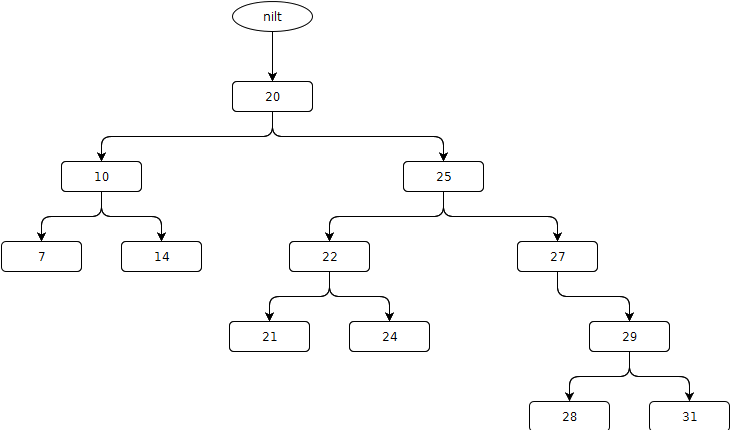
\includegraphics[scale=0.5]{w5-ressourcen/5-1-2-0.png}
\end{center}
Führen Sie nacheinander die in der Vorlesung behandelte Löschoperation für binäre Suchbäume mit den Elementen 14, 27, 25 aus.
Geben Sie den nach jeder Löschoperation erhaltenen Suchbaum an. (3 Pkt.)
\vspace{1cm}\-\\
%---------------%
%	Bearbeitung	%
%---------------%
Nach Entfernen der 14:\\
\begin{center}
	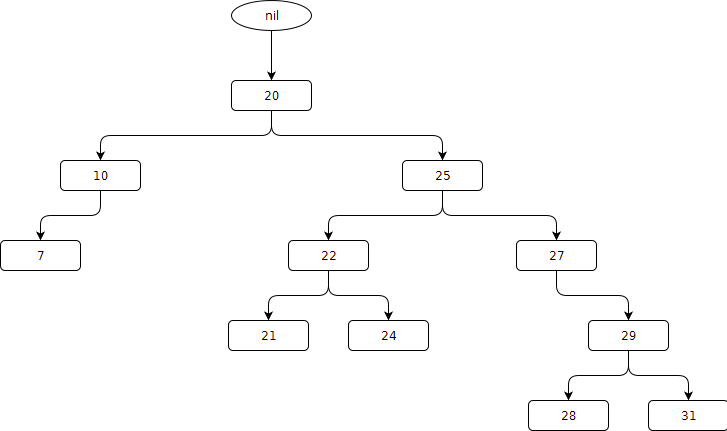
\includegraphics[scale=0.5]{w5-ressourcen/5-1-2-1.png}
\end{center}
Nach Entfernen der 27:\\
\begin{center}
	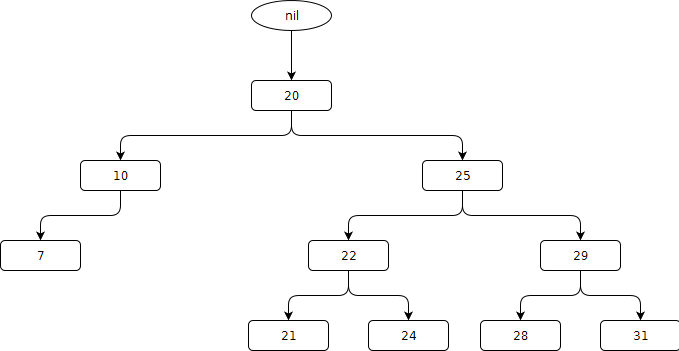
\includegraphics[scale=0.5]{w5-ressourcen/5-1-2-2.png}
\end{center}
Nach Entfernen der 25:\\
\begin{center}
	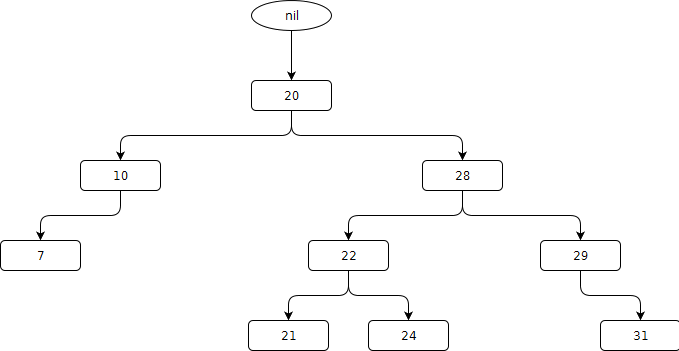
\includegraphics[scale=0.5]{w5-ressourcen/5-1-2-3.png}
\end{center}

\addcontentsline{toc}{subsection}{Übungsaufgabe 5.2}
\subsection*{Übungsaufgabe 5.2}
\label{ssec:5.2}
\begin{flushright}
\begin{Large}
[~~~~\string| ~~4~]
\end{Large}
\end{flushright}
%---------------%
%	Aufgabe		%
%---------------%
Geben Sie für die Routine \texttt{InorderTreeWalk} einen nichtrekursiven Algorithmus (3 Pkt.) und für die Routine \texttt{TreeMinimum} einen rekursiven Algorithmus (1 Pkt.) an.
Erläutern Sie in beiden Fällen unbedingt die Arbeitsweise ihres Algorithmus.

\textit{
	(Hinweis: Beide Routinen wurden in der Vorlesung behandelt.
	\texttt{InorderTreeWalk} allerdings in rekursiver, \texttt{TreeMinimum} in nichtrekursiver Darstellung.
	Für die erste Teilaufgabe hilft ein Vergleich mit der Breiten- und Tiefensuche bei Graphen.
	Für die zweite Teilaufgabe betrachte man die Routine \texttt{TreeSearch} in ihren beiden Varianten.)
}
\vspace{1cm}\-\\
%---------------%
%	Bearbeitung	%
%---------------%
\begin{codebox}
	\Procname{\texttt{inorderTreeWalk\_nichtRekursiv(x)}}
	\li $AusgabeArray = null$
	\li \texttt{TreeMinimum(x)}~~~~~~~~~~~~~~~~~~~~~~; s. Vorlesung 7 Folie 37
	\li $AusgabeArray.add(x)$
	\li \While $TreeSucessor(x) \neq nil$ \Do ~~~~~~~~~~~~~~~~~~~~~~~~~~~~~~~~~~~~~~~~; s. Vorlesung 7 Folie 47
		\li $x = TreeSucessor(x)$
		\li $AusgabeArray.add(x)$
	\li \Return $AusgabeArray$
\end{codebox}
Dieser Algorithmus sucht sich das Minimum eines Baumes und packt es in ein Array.
Danach wird sein Nachfolger gesucht und in das Array gepackt.
Sollte ein Knoten irgendwann keinen Nachfolger mehr haben, terminiert der Algorithmus und wir geben das Array aus.
\vspace{1cm}
\begin{codebox}
	\Procname{\texttt{TreeMinimum\_rekursiv(x)}}
	\li \If $links[x] \neq nil:$
		\li \texttt{TreeMinimum\_rekursiv(links[x])}
	\li \Else \Return x
\end{codebox}

Dieser Algorithmus prüft, ob der aktuelle Knoten ein linkes Kind hat.
Ist dies der Fall, wird die Methode rekursiv am linken Kind aufgerufen (das linke Kind wird von seinem Vater gefragt, was denn sein Minimum sei).
Sollte dies allerdings nicht so sein und der aktuelle Knoten besitzt kein linkes Kind, dann ist er selbst sein eigenes Minimum und damit auch das Minimum aller Knoten über ihm und wird ausgegeben.


\addcontentsline{toc}{subsection}{Übungsaufgabe 5.3}
\subsection*{Übungsaufgabe 5.3}
\label{ssec:5.3}
\begin{flushright}
\begin{Large}
[~~~~\string| ~~4~]
\end{Large}
\end{flushright}
%---------------%
%	Aufgabe		%
%---------------%
Gegeben sei ein ungerichteter Graph $G = (V, E)$ auf $n$ Knoten.
Ferner seien $s, t \in V$ Knoten, deren Distanz (ihr kürzester Abstand) echt größer als $\frac{n}{2}$ sei, d.h. $d(s, t) > n/2$.
Zeigen Sie zunächst, dass dann ein von $s$ und $t$ verschiedener Knoten $v$ existieren muss, dessen Löschung alle $s$-$t$-Pfade zerstört.
(Der Graph $G'$, der aus $G$ entsteht, wenn man $v$ löscht, enthält also keine Pfade von $s$ zu $t$ mehr.)

Geben Sie dann einen Algorithmus an, der den Knoten $v$ findet.
Können Sie einen Algorithmus angeben, der in Zeit $O(n + m)$ arbeitet?
Erläutern Sie die Arbeitsweise Ihres Algorithmus und begründen Sie seine Korrektheit sowie seine Laufzeit.

\textit{
	(Anmerkung: Die obige Fragestellung tritt bei der Untersuchung von Netzwerken auf.
	Sie besagt, dass, wenn zwei Knoten zu weit auseinander sind (nur durch viele Zwischenknoten verbunden sind), diese eine anfälligere Verbindung haben als Knoten die dichter beieinander sind.
	Obiges Resultat zeigt nämlich gerade, dass der Ausfall eines Knotens $v$ genügt, um $s$ und $t$ zu trennen.
	Allerdings ist die Aussage nicht, dass irgendein Knoten $v$ ausfallen kann und dann sofort $s$ und $t$ getrennt wären, sondern nur, dass (mindestens) ein solcher Knoten existiert.)
}
\vspace{1cm}\-\\
%---------------%
%	Bearbeitung	%
%---------------%
Sei G = (V, E) ein Graph.
Dieser Graph besitzt die Knoten s, t und v und die Bedingung, dass d(s, t) > |V|/2 gilt.
Damit enthält der kürzeste Pfad von s nach t mindestens die Hälfte aller Knoten (Genauer |V|/2 + 2 Knoten, wobei |V|/2 abgerundet wird und die + 2 durch s und t zustandekommen).
Um nun einen weiteren Pfad dieser Länge zu kreieren, muss ein Teil des bisherigen Pfades wiederverwertet werden, da sonst nicht mehr genügend freie Knoten zur Verfügung stünden.
Und für jeden weiteren Pfad werden jeweils Teile der alten Pfade wieder verwertet.
Irgendwann gehen die nicht benutzten Knoten aus und auch die Möglichkeiten übrige Knoten zu verbinden sind ausgeschöpft dann können weitere Pfade nicht generiert werden.
Alle Knoten, die nun in der Schnittmenge aller Pfade liegen, sind potentielle v Kandidaten, da jeder mögliche Pfad sie enthält - sie sozusagen die Schnittstellen aller möglichen kürzesten Pfade sind und so in jedem Pfad vorkommen müssen, damit er ein Pfad von t nach s ist.
\\
\\
Wir setzen an jeden Knoten eine hochlaufende Zahl an, so dass jeder Knoten eine eigene individuelle Zahl erhält ($(O(n)$).\\
Wir führen eine Breitensuche aus, um den kleinsten Pfad zu bestimmen ($O(n + m)$).\\
Wir führen eine Tiefensuche aus, um irgendeinen anderen Pfad zu bestimmen ($O(n + m)$).\\
Da ein Pfad von s nach t existiert, werden beide Varianten dieser Suchen einen Pfad finden.\\
Wir drehen die die Reihenfolge der Adjazenzlisten um (Für jeden Knoten n müssen alle seine Nachbarn bearbeitet werden.
Da eine Kante durch 2 "Nachbarpaare" in der Adjazenzlsite dargestellt wird, ergibt sich eine Laufzeit von $O(n + 2 * m) = O(n + m))$.\\
Wir führen eine zweite Tiefensuche durch, um einen Pfad maximal verschieden zum Zweiten zu erhalten $(O(n + m))$.\\
\\
Nun werden die 3 Listen der Suchen jeweils nach der hochlaufenden Zahl sortiert ($O(Stelligkeit * (Listenlänge + Anzahl verschiedener Stellen))$).\footnote{Quelle: s. Vorlesung 5 Folie 46 http://www.informatik.uni-hamburg.de/TGI/lehre/vl/WS1516/AuD/Folien/aud\_v5.pdf}\\
\-~~~~Die Stelligkeit dieser Zahlen ist maximal die Stelligkeit von n.
	Das Herausfinden dieser Stelligkeit geht mit konstantem Zeitaufwand.\\
\-~~~~Jede Stelle hat von Natur aus 10 mögliche Werte (0, 1, 2, 3, 4, 5, 6, 7, 8, 9)\\
\-~~~~Die Listenlänge ist im worst-case für jede Liste n.\\
\-~~~~$\Rightarrow$ Laufzeit: $3 * c * (n + 10)$. Das liegt in $O(n)$\\
Nun wird durch die 3 Listen gelaufen und jeweils verglichen, ob die Elemente in jeder dieser Liste drin sind.\\
Da es sich bei diesen Elementen um sortierte Zahlen handelt, die sich innerhalb einer Liste nicht wiederholen, muss sich der Algorithmus jedes Element jeder Liste im worst-case genau einmal anschauen (Laufzeit: $3 * n$. Dies liegt in $O(n)$).\\
Das erste gefundene Element/jedes gefundene Element (im Fall "jedes Element" muss der obige Vergleichsalgorithmus sich immer jedes Element jeder Liste anschauen, verändert aber nicht seine Laufzeit) wird in einen Knoten umgewandelt und ausgegeben (Laufzeit: $c + c$. Dies liegt in $O(c)$).\\
\\
\textbf{Gesamtlaufzeit:} $O(n) + O(n + m) + O(n + m) + O(n + m) + O(n + m) + O(n) + O(n) + O(c) = O(n + m)$\\
\textbf{Idee vollständig?:} Ja, da durch die 2 Tiefensuchen mit Umkehrung der Adjazenzliste 2 maximal voneinander unabhängige Pfade gefunden werden.
Die Schnittmenge von diesen wird in beiden Pfaden benötigt, um von s nach t zu kommen.
Durch die Breitensuche wird dann auch noch garantiert, dass es sich um einen kürzesten Pfad handelt und somit um die minimale Anzahl der Knoten.
Dies führt dazu, dass die Schnittmenge von diesem Pfad und den obigen beiden minimal ist.
Und in dieser minimalen Schnittmenge ist nun jeder Knoten ein v-Kandidat.\\
\\
\textbf{Pseudocode:}
\begin{codebox}
\Procname{\texttt{ein\_v\_knoten(Graph G, Knoten s, Knoten t)}}
	\zi //gibt einen möglichen v-Knoten aus
    \li $List~Vs = v\_knoten(G, s, t)$
    \li $index = random(Vs.length)$
    \li \Return $Vs[index]$
\end{codebox}

\begin{codebox}
\Procname{\texttt{v\_knoten(Graph G, Knoten s, Knoten t)}}
	\zi //gibt eine Liste mit allen v-Knoten aus
    \li $int i = 0$
    \li \For $Knoten n in G$
    	\Indentmore
		\li $n.zahlenwert = i$
		\li $i = i + 1$
	\End
    \li $List~A$ = \texttt{sucheKleinstenPfad(G, s, t)}
    \li $List~B$ = \texttt{sucheAnderenPfad(G, s, t)}
    \li $Graph G' = G$
    \li $G'.Adjazenzliste = reverse(G.Adjazenzliste)$
    \li $List~C$ = \texttt{sucheAnderenPfad(G', s, t)}
    
    \li $List~A'$ = \texttt{RadixSort(A nach Knoten.zahlenwert)}
    \zi // s. Vorlesung 5 Folie 46; Link: http://www.informatik.uni-hamburg.de/TGI/lehre/vl/
    \zi // WS1516/AuD/Folien/aud\_v5.pdf
    \li $List~B'$ = \texttt{RadixSort(B nach Knoten.zahlenwert)}
    \li $List~C'$ = \texttt{RadixSort(C nach Knoten.zahlenwert)}

    \li $List~ErgebnisListe = new~List$
    \li $aktuellerKnoten = new~Knoten$
    \li $indexA = 0$
    \li $indexB = 0$
    \li $indexC = 0$

    \li \While $A'.length > indexA$ \textbf{and} $B'.length > indexB$ \textbf{and} $C'.length > indexC:$
    \zi //echt größer, da der Index ab 0 beginnt
    	\Indentmore
        \li $aktuellerKnoten = A'[indexA]$
        \li \If $aktuellerKnoten < B'[indexB]$
        	\Indentmore
            \li $indexA = indexA + 1$
        \li \Else \If $aktuellerKnoten > B'[indexB]$
            \li $indexB = indexB + 1$
        \li \Else
        \zi //falls aktuellerKnoten == B'[indexB] ist
            \li \If $aktuellerKnoten < C'[indexC]$
            	\Indentmore
				\li $indexA = indexA + 1$
			\li \Else \If $aktuellerKnoten > C'[indexC]$
				\li $indexC = indexC + 1$
			\li \Else
			\zi //falls aktuellerKnoten == C'[indexC] ist
				\li $ErgebnisListe.add(aktuellerKnoten)$
				\li $indexA = indexA + 1$
			\End
		\End
	\End
    \li \Return $ErgebnisListe$
\end{codebox}    

\begin{codebox}
\Procname{\texttt{sucheAnderenPfad(Graph G, Knoten s, Knoten t)}}
	\zi //gibt einen Pfad von s nach t aus aus
    \li \texttt{Tiefensuche(G, s)}
    \li \Return \texttt{bauePfad(G, s, t)}
\end{codebox}

\begin{codebox}
\Procname{\texttt{bauePfad(Graph G, Knoten s, Knoten t)}}
	\zi //baut gegeben einen durchsuchten Graphen einen Pfad von s nach t
	\zi //(s und t sind nicht in dem Pfad enthalten um später nicht in der Schnittmenge zu landen)
    \li $Knoten~n = t.parent$
    \li $List~A = new List$
    \li \While $!(n == s)$
        \li $A.add(n)$
        \li $n = n.parent$
    \li \li Return $A$
\end{codebox}    

\begin{codebox}
\Procname{sucheKleinstenPfad(Graph G, Knoten s, Knoten t)}
	\zi // gibt einen kürzesten Pfad von s nach t aus
    \li \texttt{Breitensuche(G, s)}
    \li \Return \texttt{bauePfad(G, s, t)}
\end{codebox}

\begin{codebox}
\Procname{Tiefensuche(Graph G, Knoten wurzel)}
	\zi // führt eine Tiefensuche auf dem Graphen durch
    \li \For $Knoten~n~in~G$
    	\Indentmore
        \li $n.entdeckt = false$
        \li $n.parent = NIL$
    \End
    \li $Stack S = new Stack$
    \li \texttt{S.push(wurzel)}
    \li $Knoten~aktuellerKnoten = NULL$
    \li \While $!(S is empty)$
    	\Indentmore
        \li $aktuellerKnoten$ = \texttt{S.pop()}
        \li \If $aktuellerKnoten.entdeckt == false$
        	\Indentmore
            \li $aktuellerKnoten.entdeckt = true$
        \End
	    \li \For $Knoten~m~in~aktuellerKnoten.AdjazenzListe$
	    	\Indentmore
	        \li \texttt{S.push(m)}
	    \End
		\li $m.parent = aktuellerKnoten$
	\End
\end{codebox}

\begin{codebox}
\Procname{Breitensuche(Graph G, Knoten wurzel)}
	\zi // führt eine Breitensuche auf dem Graphen durch
    \li \For $Knoten~n~in~G$
    	\Indentmore
        \li $n.distanz = INFINITY$
	    \li $n.parent = NIL$
	\End
    \li $Queue~Q = new~Queue$
    \li $wurzel.distanz = 0$
    \li $q.enqueque(wurzel)$
    \li $Knoten~aktuellerKnoten = NULL$
    \li \While $!(Q is empty)$
    	\Indentmore
        \li $aktuellerKnoten = Q.dequeue()$
        \li \For $Knoten~m~in~aktuellerKnoten.Adjazenzliste$
        	\Indentmore
            \li \If $m.distanz == INFINITY$
	            \Indentmore
                \li $m.distanz = aktuellerKnoten.distanz + 1$
                \li $m.parent = aktuellerKnoten$
                \li $q.enqueue(m)$
            \End
        \End
    \End
\end{codebox}



\addcontentsline{toc}{subsection}{Übungsaufgabe 5.4}
\subsection*{Übungsaufgabe 5.4}
\label{ssec:5.4}
\begin{flushright}
\begin{Large}
[~~~~\string| ~~4~]
\end{Large}
\end{flushright}
\addcontentsline{toc}{subsubsection}{Aufgabe 5.4.1}
\subsubsection*{Aufgabe 5.4.1}
\label{sssec:5.4.1}
%---------------%
%	Aufgabe		%
%---------------%
Im Problem \texttt{Big-Clique} ist ein ungerichteter Graph $G$ gegeben.
Die Frage ist, ob $G$ eine Clique enthält, die aus mindestens $\frac{n}{2}$ Knoten besteht (wobei $n$ die Anzahl der Knoten von $G$ ist).
Zeigen Sie, dass \texttt{Big-Clique} NP-vollständig ist. (2 Pkt.)
\vspace{1cm}\-\\
%---------------%
%	Bearbeitung	%
%---------------%
Big-Clique liegt in NP.\\
Verifikationsalgorithmus, der die Richtigkeit eines gegebenen Zertifikates in polynomialzeit überprüft:\\
\-~~~~Unser Zertifikat: Eine Menge an Knoten - unsere Clique - und der Graph\\
\-~~~~Wir schauen in der Adjazenzliste nach, ob zu jedem gegebenen Knoten, zu allen anderen gegebenen Knoten eine Kante existiert.
	Ist dies der Fall, ist das Zertifikat richtig, sonst nicht.\\
Big-Clique liegt in NPH.\\
Reduktion eines Algorithmusses aus NPH auf Big-Clique:\\
\-~~~~Wir nehmen Clique(G, k): G = (V, K) Graph, k = Größe der Clique\\
\-~~~~Wenn unser k größer oder gleich |V|/2 ist, geben wir das Problem einfach in Big-Clique.\\
\-~~~~Ist es allerdings kleiner, fügen wir für jeden Knoten, der uns auf |V|/2 fehlt, 2 Knoten an den Graphen an, die wir jeweils mit Kanten zu allen anderen Knoten versehen.\\
\-~~~~Diesen neuen Graphen fügen wir in den Automaten ein, der Big-Clique löst und geben die Lösung als unsere Lösung für unser Clique-Problem aus.\\
Da wir beides obere haben, folgt daraus: Big-Clique liegt in NPC


\addcontentsline{toc}{subsubsection}{Aufgabe 5.4.2}
\subsubsection*{Aufgabe 5.4.2}
\label{sssec:5.4.2}
%---------------%
%	Aufgabe		%
%---------------%
Geben Sie unter der Annahme $P = NP$ einen deterministischen Algorithmus an, der in polynomieller
Zeit zu einem ungerichteten Graphen $G$ eine maximal große Clique bestimmt. (2 Pkt.)
\vspace{1cm}\-\\
%---------------%
%	Bearbeitung	%
%---------------%
Verifikationsalgorithmus, der die Richtigkeit eines gegebenen Zertifikates in polynomialzeit überprüft:\\
\-~~~~Unser Zertifikat: Eine Menge an Knoten - unsere größte mögliche Clique - und der Graph\\
\-~~~~Wir geben unseren Graph und die Zahl k = |Menge an Knoten| + 1 in Clique.\\
\-~~~~Wenn Clique wahr ausgibt, ist das Zertifikat falsch, da eine größere Clique existiert.\\
\-~~~~Dies läuft in polynomialzeit, da P = NP angenommen wird.\\
Durch diesen Verifikationsalgorithmus ist unser Problem in NP.\\
Unter der Annahme P = NP existiert allerdings auch ein P-Algorithmus und dieser ist deterministisch.

\newpage
%#+--------------------------------------------------+#%
%#+						ZETTEL 5				     +#%
%#+--------------------------------------------------+#%
\addcontentsline{toc}{section}{Zettel vom 10. 12. -- Abgabe: 04. 01. 2016}
\section*{Zettel vom 10. 12. -- Abgabe: 04. 01. 2016}
\sus{6.1}
\points{10}
%---------------%
%	Aufgabe	    %
%---------------%
\begin{center}
\begin{tikzpicture}[->,>=stealth',shorten >=1pt,auto,semithick]
\node	[state]	(s)						{S};
\node	[state]	(b)	[right=2cm of s]	{B};
\node	[state]	(a)	[above=1cm of b]	{A};
\node	[state]	(c)	[below=1cm of b]	{C};
\node	[state]	(e)	[right=2cm of b]	{E};
\node	[state]	(d)	[above=1cm of e]	{D};
\node	[state]	(f)	[below=1cm of e]	{F};
\node	[state]	(g)	[right=2cm of e]	{G};

\path
	(s)	edge	[above]	node	[align=center]	{1}	(a)
	(s)	edge			node	[align=center]	{4}	(b)
	(s)	edge			node	[align=center]	{9}	(c)
	(a)	edge			node	[align=center]	{1}	(d)
	(a)	edge	[above]	node	[align=center]	{5}	(e)
	(b)	edge			node	[align=center]	{5}	(a)
	(b)	edge			node	[align=center]	{2}	(e)
	(c)	edge			node	[align=center]	{1}	(b)
	(c)	edge			node	[align=center]	{6}	(f)
	(d)	edge	[below]	node	[align=center]	{1}	(b)
	(d)	edge			node	[align=center]	{15}(g)
	(e)	edge			node	[align=center]	{3}	(c)
	(f)	edge			node	[align=center]	{1}	(g)
	(g)	edge			node	[align=center]	{4}	(e)
;
\end{tikzpicture}
\end{center}
Betrachten Sie obigen Graphen $G$.
Wenden Sie jeweils das verlangte Verfahren an bzw. beantwortet Sie die Frage oder begründen Sie, warum dies nicht nicht.
(Bei den ersten sechs Teilaufgaben spielen die Kantengewichte keine Rolle.)

\sss{6.1.1}
%---------------%
%	Aufgabe	    %
%---------------%
Ermittel Sie mit der Breitensuche einen Breitensuchbaum.
Starten Sie den Algorithmus bei $s$. (1 Pkt.)
\vspace{1cm}\-\\
%---------------%
%	Bearbeitung %
%---------------%
Ergebnis der Breitensuche:

S A B C D E F G\\
BFS-Baum:
\begin{center}
	\includegraphics[scale=0.5]{w6-ressourcen/6-1-BFS-Tree.png}
\end{center}
\sss{6.1.2}
%---------------%
%	Aufgabe	    %
%---------------%
Ist das Ergebnis der Breitensuche eindeutig? (1 Pkt.)
\vspace{1cm}\-\\
%---------------%
%	Bearbeitung %
%---------------%
Ja, ist es, da die Reihenfolge der Kanten, die gewählt werden, gegeben ist durch die Struktur der Adjazenzmatrix des Graphen.
Zumindest ist dies der Fall bei den bisher im Modul gegebenen Algorithmen.
Liegt keine Adjazenzmatrix vor oder arbeitet ein Algorithmus mit einer Modifikation der BFS, so kann es, gegeben es gibt mehrere gültige Breitensuchbäume, dazu kommen, dass unterschiedliche Ergebnisse zurückgegeben werden.

\sss{6.1.3}
%---------------%
%	Aufgabe	    %
%---------------%
Ermitteln Sie mit der Tiefensuche einen Tiefensuchwald und insb. die Zeiten $d[v]$ und $f[v]$ für jeden Knoten $v$.
Starten Sie den Algorithmus wieder bei $s$. (1 Pkt.)
\vspace{1cm}\-\\
%---------------%
%	Bearbeitung %
%---------------%
\begin{minipage}[t]{0.42\textwidth}
\begin{tabular}{l|l||c|c}
\textbf{Ergebnis}	&	\textbf{Stack}	&	$d[v]$	&	$f[v]$	\\ \hline
/			&	S			&	--	&	--	\\
S			&	SA			&	S:0	&	--	\\
SA			&	SAD			&	A:1	&	--	\\
SAD			&	SADB		&	D:2	&	--	\\
SADB		&	SADBE		&	B:3	&	--	\\
SADBE		&	SADBEC		&	E:4	&	--	\\
SADBEC		&	SADBECF		&	C:5	&	--	\\
SADBECF		&	SADBECFG	&	F:6	&	--	\\
SADBECFG	&	SADBECFG	&	G:7	&	--	
\end{tabular}
\end{minipage}
\begin{minipage}[t]{0.42\textwidth}
\begin{tabular}{l|l||c|c}
\textbf{Ergebnis}	&	\textbf{Stack}	&	$d[v]$	&	$f[v]$	\\ \hline
SADBECFG	&	SADBECF	&	--	&	G:8		\\
SADBECFG	&	SADBEC	&	--	&	F:9		\\
SADBECFG	&	SADBE	&	--	&	C:10	\\
SADBECFG	&	SADB	&	--	&	E:11	\\
SADBECFG	&	SAD		&	--	&	B:12	\\
SADBECFG	&	SA		&	--	&	D:13	\\
SADBECFG	&	S		&	--	&	A:14	\\
SADBECFG	&	/		&	--	&	S:15	
\end{tabular}
\end{minipage}
\begin{minipage}[t]{0.22\textwidth}
\begin{tabular}{c||c|r}
\textbf{Knoten}	&	$d[v]$	&	$f[v]$	\\	\hline
S	&	0	&	15\\
A	&	1	&	14\\
B	&	3	&	12\\
C	&	5	&	10\\
D	&	2	&	13\\
E	&	4	&	11\\
F	&	6	&	9\\
G	&	7	&	8
\end{tabular}
\end{minipage}

\sss{6.1.4}
%---------------%
%	Aufgabe	    %
%---------------%
Geben Sie eine topologische Sortierung des Graphen $G$ an. (1 Pkt.)
\vspace{1cm}\-\\
%---------------%
%	Bearbeitung %
%---------------%
Es ist nicht möglich, eine topologische Sortierung für $G$ anzugeben, da $G$ zyklisch ist und somit unabhängig von der gewählten Reihenfolge keine Möglichkeit besteht, rückwärtige Kanten zu vermeiden.

\sss{6.1.5}
%---------------%
%	Aufgabe	    %
%---------------%
Bestimmen Sie mit dem Algorithmus aus der Vorlesung die starken Zusammenhangskomponenten von $G$.
Geben Sie dazu das Ergebnis von $DFS(G)$ und $DFS(G^T)$ sowie die starken Zusammenhangskomponenten an. (1 Pkt.)
\vspace{1cm}\-\\
%---------------%
%	Bearbeitung %
%---------------%
$DFS(G):$ s. 6.1.3.\\
$DFS(G^T):$ nicht möglich, da keine topologische Sortierung vorliegt.\\
Starke Zusammenhangskomponenten:

[S], [A,B,C,D,E,F,G]

\sss{6.1.6}
%---------------%
%	Aufgabe	    %
%---------------%
Geben Sie den Komponentengraphen von $G$ an. (1 Pkt.)
\vspace{1cm}\-\\
%---------------%
%	Bearbeitung %
%---------------%
Der Übersicht halber wurden die Kantengewichte, da sie für diese Aufgabe ohnehin irrelevant sind, weggelassen.
\begin{center}
	\includegraphics[scale=0.6]{w6-ressourcen/6-1-6-cpg.png}
\end{center}
\sss{6.1.7}
%---------------%
%	Aufgabe	    %
%---------------%
Interpretieren Sie $G$ nun als ungerichteten Graphen.
Wenden Sie den Algorithmus von Kruskal an, um einen minimalen Spannbaum zu bestimmen.
(Es genügt hier anzugeben welche Kanten in den minimalen Spannbaum aufgenommen werden und in welcher Reihenfolge dies geschieht!) (1 Pkt.)
\vspace{1cm}\-\\
%---------------%
%	Bearbeitung %
%---------------%
\textbf{Schritt 1:} Hinzufügen aller Kanten mit Gewicht 1.\\
$\{(S,A),(A,D),(B,D),(B,C),(F,G)\}$
\begin{center}
	\includegraphics[scale=.6]{w6-ressourcen/6-1-7-1.png}
\end{center}
\textbf{Schritt 2:} Hinzufügen aller Kanten mit Gewicht 2.\\
$\{(B,E)\}$
\begin{center}
	\includegraphics[scale=.6]{w6-ressourcen/6-1-7-2.png}
\end{center}
\textbf{Schritt 3:} Kanten mit Gewicht 3 sind redundant.
Fahre fort mit Kanten mit Gewicht 4.\\
$\{(E,G)\}$
\begin{center}
	\includegraphics[scale=.6]{w6-ressourcen/6-1-7-3.png}
\end{center}

\sss{6.1.8}
%---------------%
%	Aufgabe	    %
%---------------%
Bestimmen Sie mit dem Algorithmus von Dijkstra kürzeste Pfade von $s$ zu allen anderen Knoten.
Geben Sie hierzu jeweils den Graph mit den Werten von $d[v]$ nach jeder Iteration der while-Schleife an und machen Sie $\pi[v]$ z.B. durch dickere Kanten deutlich. (2 Pkt.)
\vspace{1cm}\-\\
%---------------%
%	Bearbeitung %
%---------------%
Sei $v \in V(G)$.
Dann ordnet $d(v)$ jedem Knoten seine Distanz zum Startknoten zu.
Sei desweiteren die Startdistanz jedes Knoten zum Startknoten zunächst $\infty$.
Außerdem werden fertig bearbeitete Knoten mit \textcolor{red}{roter} Schrift markiert, der als nächstes geprüfte Knoten in \textcolor{green}{grüner} Schrift.
\newpage
\begin{enumerate}
	\item \textbf{Anfang}\\
	\begin{minipage}[t]{0.48\textwidth}
		\begin{tabular}{l||c|c|c|c|c|c|c|c}
			$v$		&	\textcolor{green}{S}	&	A	&	B	&	C	&	D	&	E	&	F	&	G	\\	\hline
			$d(v)$	&	0						&	$\infty$	&	$\infty$	&	$\infty$	&	$\infty$	& $\infty$	&	$\infty$	&	$\infty$
		\end{tabular}
	\end{minipage}
	\begin{minipage}[t]{0.48\textwidth}
		\includegraphics[scale=0.5]{w6-ressourcen/6-1-8-0.png}
	\end{minipage}
	
	\item \textbf{S}\\
	\begin{minipage}[t]{0.48\textwidth}
		\begin{tabular}{l||c|c|c|c|c|c|c|c}
			$v$		&	\textcolor{red}{S}	&	\textcolor{green}{A}	&	B	&	C	&	D	&	E	&	F	&	G	\\	\hline
			$d(v)$	&	0					&	1	&	4	&	9	&	$\infty$	&	$\infty$	&	$\infty$	&	$\infty$
		\end{tabular}\\\\
		Kanten:\\
		$(s,a),(s,b),(s,c)$
	\end{minipage}
	\begin{minipage}[t]{0.48\textwidth}
		\includegraphics[scale=0.5]{w6-ressourcen/6-1-8-1.png}
	\end{minipage}
	
	\item \textbf{A}\\
	\begin{minipage}[t]{0.48\textwidth}
		\begin{tabular}{l||c|c|c|c|c|c|c|c}
			$v$		&	\textcolor{red}{S}	&	\textcolor{red}{A}	&	B	&	C	&	\textcolor{green}{D}	&	E	&	F	&	G	\\	\hline
			$d(v)$	&	0					&	1					&	4	&	9	&	2	&	6	&	$\infty$	&	$\infty$
		\end{tabular}\\\\
		Kanten:\\
		$(s,a),(s,b),(s,c),(a,d),(a,e)$
	\end{minipage}
	\begin{minipage}[t]{0.48\textwidth}
		\includegraphics[scale=0.5]{w6-ressourcen/6-1-8-2.png}
	\end{minipage}
	
	\item \textbf{D}\\
	\begin{minipage}[t]{0.48\textwidth}
		\begin{tabular}{l||c|c|c|c|c|c|c|c}
			$v$		&	\textcolor{red}{S}	&	\textcolor{red}{A}	&	\textcolor{green}{B}	&	C	&	\textcolor{red}{D}&	E	&	F	&	G	\\	\hline
			$d(v)$	&	0	&	1	&	4	&	9	&	2	&	6	&	$\infty$	&	17
		\end{tabular}\\\\
		Kanten:\\
		$(s,a),(s,c),(a,d),(a,e),(d,b),(d,g)$
	\end{minipage}
	\begin{minipage}[t]{0.48\textwidth}
		\includegraphics[scale=0.5]{w6-ressourcen/6-1-8-3.png}
	\end{minipage}
	
	\item \textbf{B}\\
	\begin{minipage}[t]{0.48\textwidth}
		\begin{tabular}{l||c|c|c|c|c|c|c|c}
			$v$		&	\textcolor{red}{S}	&	\textcolor{red}{A}	&	\textcolor{red}{B}	&	C	&	\textcolor{red}{D}	&	\textcolor{green}{E}	&	F	&	G	\\	\hline
			$d(v)$	&	0	&	1	&	3	&	9	&	2	&	5	&	$\infty$	&	17
		\end{tabular}\\\\
		Kanten:\\
		$(s,a),(s,b),(s,c),(a,d),(a,e)$
	\end{minipage}
	\begin{minipage}[t]{0.48\textwidth}
		\includegraphics[scale=0.5]{w6-ressourcen/6-1-8-4.png}
	\end{minipage}
	
	\item \textbf{E}\\
	\begin{minipage}[t]{0.48\textwidth}
		\begin{tabular}{l||c|c|c|c|c|c|c|c}
			$v$		&	\textcolor{red}{S}	&	\textcolor{red}{A}	&	\textcolor{red}{B}	&	\textcolor{green}{C}	&	\textcolor{red}{D}	&	\textcolor{red}{E}	&	F	&	G	\\	\hline
			$d(v)$	&	0	&	1	&	3	&	8	&	2	&	5	&	$\infty$	&	17
		\end{tabular}\\\\
		Kanten:\\
		$(s,a),(a,d),(d,b),(d,g),(b,e),(e,c)$
	\end{minipage}
	\begin{minipage}[t]{0.48\textwidth}
		\includegraphics[scale=0.5]{w6-ressourcen/6-1-8-5.png}
	\end{minipage}
	
	\item \textbf{C}\\
	\begin{minipage}[t]{0.48\textwidth}
		\begin{tabular}{l||c|c|c|c|c|c|c|c}
			$v$		&	\textcolor{red}{S}	&	\textcolor{red}{A}	&	\textcolor{red}{B}	&	\textcolor{red}{C}	&	\textcolor{red}{D}	&	\textcolor{red}{E}	&	\textcolor{green}{F}	&	G	\\	\hline
			$d(v)$	&	0	&	1	&	3	&	8	&	2	&	5	&	14	&	17
		\end{tabular}\\\\
		Kanten:\\
		$(s,a),(a,d),(d,b),(d,g),(b,e),(e,c),(c,f)$
	\end{minipage}
	\begin{minipage}[t]{0.48\textwidth}
		\includegraphics[scale=0.5]{w6-ressourcen/6-1-8-6.png}
	\end{minipage}
	
	\item \textbf{F}\\
	\begin{minipage}[t]{0.48\textwidth}
		\begin{tabular}{l||c|c|c|c|c|c|c|c}
			$v$		&	\textcolor{red}{S}	&	\textcolor{red}{A}	&	\textcolor{red}{B}	&	\textcolor{red}{C}	&	\textcolor{red}{D}	&	\textcolor{red}{E}	&	\textcolor{red}{F}	&	\textcolor{green}{G}	\\	\hline
			$d(v)$	&	0	&	1	&	3	&	8	&	2	&	5	&	14	&	15
		\end{tabular}\\\\
		Kanten:\\
		$(s,a),(a,d),(d,b),(b,e),(e,c),(c,f),(f,g)$
	\end{minipage}
	\begin{minipage}[t]{0.48\textwidth}
		\includegraphics[scale=0.5]{w6-ressourcen/6-1-8-7.png}
	\end{minipage}
	
	\item \textbf{G}\\
	\begin{minipage}[t]{0.48\textwidth}
		\begin{tabular}{l||c|c|c|c|c|c|c|c}
			$v$		&	\textcolor{red}{S}	&	\textcolor{red}{A}	&	\textcolor{red}{B}	&	\textcolor{red}{C}	&	\textcolor{red}{D}	&	\textcolor{red}{E}	&	\textcolor{red}{F}	&	\textcolor{red}{G}	\\	\hline
			$d(v)$	&	0	&	1	&	3	&	8	&	2	&	5	&	14	&	15
		\end{tabular}\\\\
		Kanten:\\
		$(s,a),(a,d),(d,b),(b,e),(e,c),(c,f),(f,g)$
	\end{minipage}
	\begin{minipage}[t]{0.48\textwidth}
		\includegraphics[scale=0.5]{w6-ressourcen/6-1-8-7.png}
	\end{minipage}
\end{enumerate}

\sss{6.1.9}
%---------------%
%	Aufgabe	    %
%---------------%
Betrachten Sie den Sourcecode von Dijkstras Algorithmus und vom Algorithmus von Prim.
Was ist der hauptsächliche Unterschied der beiden Algorithmen bei der Ausführung? (1 Pkt.)
\vspace{1cm}\-\\
%---------------%
%	Bearbeitung %
%---------------%
Während Dijkstra die Entfernung jedes Knotens zum Startknoten speichert, enthalten die Knoten nach Prim jeweils nur die Entfernung zum Vorgängerknoten.
Dieser Unterschied wird durch Dijkstra's \texttt{Relax} in Zeile 8ff\footnote{Foliensatz 9, Version 03.01.2016, Seite 119} hervorgerufen (Dieser \texttt{if}-Block ist äquivalent zur Funktion \texttt{Relax} von der Seite vorher).

\sus{6.2}
\points{6}
\sss{6.2.1}
%---------------%
%	Aufgabe	    %
%---------------%
Sei $G = (V,E)$ ein ungerichteter Graph.
Bei einer $k$-Färbung von $G$ wird jedem Knoten $v \in V$ eine Farbe $c \in [k] = \{1,2,\dots,k\}$ zugewiesen.
Die Färbung ist korrekt, wenn zwei benachbarte Knoten nie die gleiche Farbe haben.
Formal ist eine \textit{k-Färbung} dann also eine Abbildung $f : V \rightarrow [k]$ und eine \textit{korrekte k-Färbung} erfüllt $f(x) \neq f(y)$ für jede Kante $\{x,y\} \in E$.
Wir definieren folgendes Problem:
\[
	k-col = \{\langle G \rangle | G \text{ besitzt eine korrekte } k\text{-Färbung}\}
\]
Angenommen Sie wissen, dass 3-col \textit{NP}-vollständig ist.
Zeigen Sie, dass auch 8-col \textit{NP}-vollständig ist. (2 Pkt.)
\vspace{1cm}\-\\
%---------------%
%	Bearbeitung %
%---------------%
Sei das Zertifikat eine Menge bestehend aus einem Graphen $G=(V,E)$ und einer Färbungsfunktion $f$.
Die Prüfung des korrekten Ergebnisses der Funktion in Form von $f(x) \neq f(y)$ für zwei benachbarte Knoten $x,y \in V$ lässt sich in polynomieller Zeit erledigen, womit 8-col in NP liegt.\\
\\
\textbf{Reduktion}\\
Es wird nach Aufgabenstellung 3-col auf 8-col reduziert.\\
Nach Aufgabenstellung ist bekannt, dass 3-col in NP liegt.\\
\\
Sei die Gruppe $H$ eine Menge von Knoten, die eine erfüllende Belegung von 3-col darstellt.
Zu $H$ wird ein Knoten hinzugefügt, der paarweise mit allen drei Knoten aus $H$ verbunden wird.
Da der neue Knoten mit allen anderen Knoten verbunden ist, muss er eine Farbe erhalten, die bisher nicht vergeben ist.
$H'$ ist nun eine erfüllende Belegung für 4-col und jede 3 Knoten aus $H$ sind eine erfüllende Belegung für 3-col.
Dies wird wiederholt, bis $H'_neu$ 8 Knoten vorweist.
Für jede k Knoten gilt hierbei, dass es sich um eine erfüllende Belegung für k-col handelt, und jede Auswahl aus k-1 Knoten aus $H$ eine erfüllende Belegung für (k-1)-col ist.
Diese Erweiterung liegt in $\mathcal{O}(k-|V_{H_0}|)$.

\sss{6.2.2}
%---------------%
%	Aufgabe	    %
%---------------%
Wir betrachten das folgende Spiel: Auf eiem Feld mit $n$ Spalten, $n$ Zeilen und $n \times n $ Feldern können auf jeder der $n^2$ Positionen entweder ein weißer oder ein schwarzer Stein liegen oder das Feld kann leer sein.
Eine Anfangsmarkierung besteht aus einer Zuweisung von Spielsteinen zu Feldern.
Das Spiel wird dann (alleine) gespielt, indem beliebig viele Steine entfernt werden.
Ziel ist es, dass jede Spalte nur noch Steine einer Farbe enthält (oder leer ist) und jede Zeile mindestens einen Stein enthält.
Ob man dieses Ziel erreichen kann (und damit gewinnt), hängt von der Anfangsmarkierung ab.
Die Eingabe ist ein Spiel $S$ bestehend aus dem Feld und der Anfangsmarkierung (für das Feld reicht die Zahl n).
Die Eingabe wird akzeptiert, wenn $S$ gewonnen werden kann.
Zeigen Sie, dass dieses Problem \textit{NP}-vollständig ist. (4 Pkt.)
\vspace{1cm}\-\\
%---------------%
%	Bearbeitung %
%---------------%
\textbf{Reduktion von 3KNF auf Kreuzgo\footnote{Wir haben das Spiel in Ermangelung eines Namen so getauft}:}\\
Eine Spalte wird als Klausel interpretiert, die dann wahr ist, wenn für jedes Feld gilt:
\[
    ((schwarz \land \lnot weiss) \lor (\lnot schwarz \land weiss) \lor null)
\]
je nachdem, ob der erste gefundene Stein in der Spalte schwarz oder weiß ist.\\
Ebenso wird eine Zeile als Klausel interpretiert, die dann wahr ist, wenn für mindestens ein Feld gilt:
\[
    (schwarz \lor weiss \lor \lnot null)
\]
Diese Belegung muss für jede Zeile bzw. jede Spalte respektive gelten; die einzelnen Klauseln sind konjunkt.\\
Gibt es eine erfüllende Belegung für die dadurch entstehende KNF, so ist diese Lösung auch eine Lösung für Kreuzgo.



%#+-------------------------------------------------+#%
%#+						ZETTEL 8					+#%
%#+-------------------------------------------------+#%
\newpage
\addcontentsline{toc}{section}{Zettel vom 06. 01. -- Abgabe: 18. 01. 2016}
\section*{Zettel vom 06. 01. -- Abgabe: 18. 01. 2016}
\points{16}
\sus{7.1}
\sss{7.1.1}
%---------------%
%	Aufgabe	    %
%---------------%
Sei $G=(V,E)$ ein Flussnetzwerk mit Kapazitätsfunktion $c,u,v \in V$ und $f$ ein Fluss in $G$.
Beweisen Sie die folgende Gleichung:
\[
	c_f(u,v)+c_f(v,u)=c(u,v)+c(v,u),
\]
wobei$c_f$ wie in der Vorlesung definiert ist.
Geben Sie bei jedem Schritt eine Begründung an (z.B. folgt aus der Definition o.ä.).
Was ist die Aussage der obigen Gleichung? (2 Pkt.)\\
\vspace{1cm}
%---------------%
%	Bearbeitung %
%---------------%

\begin{tabular}{llll}
	$c_f(u,v)+c_f(v,u)$&=&$c(u,v)-f(u,v)+c(v,u)-f(v,u)$&$s. Vl. 10 S. 24$\\
	&=&$c(u,v)+c(v,u)-f(u,v)-f(v,u)$&$Kommutativgesetz$\\
	&=&$c(u,v)+c(v,u)-f(u,v)--f(u,v)$&$s. Vl. 10 S. 17 Punkt 2$\\
	&=&$c(u,v)+c(v,u)-f(u,v)+f(u,v)$&$doppelte~Negation$\\
	&=&$c(u,v)+c(v,u)\qed$&$-a+a=a-a=0$
\end{tabular}\\
\textbf{Aussage:}
Die Restkapazität von $(u,v)$ plus die Restkapazität der Gegenrichtung $(v,u)$ ist gleich der Kapazität von $(u,v)$ plus die Kapazität der Gegenrichtung $(v,u)$.
\sss{7.1.2}
%---------------%
%	Aufgabe	    %
%---------------%
Seien $u$ und $v$ Knoten in einem Flussnetzwerk $G=(V,E)$ derart, dass $(u,v) \not\in E\text{ und }(v,u)\not\in E$ gilt.
Beweisen Sie, dass dann $f(u,v)=f(v,,u)=0$ gilt.
Begründen Sie auch hier Ihre Schritte. (2 Pkt.)\\
\vspace{1cm}
%---------------%
%	Bearbeitung %
%---------------%

\begin{enumerate}
	\item[A] Da $(u,v) \not \in E$, gilt nach Vl. 10 S. 4 $c(u,v)=0$.
	\item[B] Da außerdem nach Vl. 10 S. 5 $f(u,v)\leq c(u,v)$ gilt, muss $f(u,v)\leq 0$ sein.
	\item[A2] [A] gelte auch für $(v,u)\not \in E$.
	\item[B2] [B] gelte auch für $(v,u)\not \in E$.
	\item[C] Nach Asymmetrie (vgl. Vl. 10 S. 5) gilt $f(u,v)=f(v,u)$
	\item[D] Nach [B], [B2], [C]: $0\geq f(u,v) = f(v,u) \leq 0$
	\item[E] $\Rightarrow 0=f(u,v)=f(v,u)$
\end{enumerate}


\sss{7.1.3}
%---------------%
%	Aufgabe	    %
%---------------%
Sei $G=(V,E)$ ein Flussnetzwerk und $f$ ein Fluss in $G$.
Seien $X,Y,Z \subseteq V$ mit $X \cap Y = \emptyset$.
Beweisen Sie
\[
	\begin{array}{ccc}
		f(X\cup Y,Z)& = &f(X,Z)+f(Y,Z)\\
		f(Z,X\cup Y)& = &f(Z,X)+f(Z,Y)
	\end{array}
\]
Begründen Sie auch hier ihre Schritte.
Warum ist die Bedingung $X \cap Y = \emptyset$ nötig? (4 Pkt.)\\
\vspace{1cm}
%---------------%
%	Bearbeitung %
%---------------%

\begin{enumerate}
	\item Da $X \cap Y=\emptyset$, kann $X \cup Y = X + Y$ gesetzt werden 
\end{enumerate}
\begin{tabular}{llll}
$f(X\cup Y), Z$ &=&$\underset{x,y\in X\cup Y}{\sum}\underset{z \in Z}{\sum}f(xy,z)$&$Vl. 10 S. 16; 1.$\\
	&=&$\underset{x,y\in X + Y}{\sum}\underset{z \in Z}{\sum}f(xy,z)$&$Attributivgesetz$\\
	&=&$\underset{x \in X}{\sum}\underset{z \in Z}{\sum}f(x,z) + \underset{y \in Y}{\sum}\underset{z \in Z}{\sum}f(y,z)$&$Vl. 10 S. 16$\\
	&=&$f(X,Z)+f(Y,Z)\qed$
\end{tabular}\\\\
Für $f(Z,X\cup Y) = f(Z,X)+f(Z,Y)$: Die Umformung erfolgt im hinteren Teil des Ausdruckes; der Weg ist identisch.\\
\\
$X \cap Y=\emptyset$ ist erforderlich für $X \cup Y = X + Y$.

\sss{7.1.4}
%---------------%
%	Aufgabe	    %
%---------------%
Betrachten Sie das folgende Flussnetzwerk:
\begin{center}
	\includegraphics[scale=.7]{w7-ressourcen/7-1-4-0.png}
\end{center}
Bestimmen Sie mit dem Algorithmus von Edmonds-Karp einen maximalen Fluss und diesem Netzwerk.
Geben Sie dazu stets als erstes den Erweiterungspfad im Restnetzwerk an (beachten Sie, dass das erste Restnetzwerk dem gegebenen Flussnetzwerk entspricht!), indem Sie einfach die Knoten des Pfades auflisten (z.B. $SABC$ für den Pfad von $S$ nach $C$ über $A$ und $B$= und dn Wert des Flusses angeben.
Zeichnen Sie dann das obige Flussnetzwerk mit dem ermittelten gesamten Fluss.
Als drittes zeichnen Sie das neue Restnetzwerk.
Dann geben Sie sofern möglich einen neuen Erweiterungspfad an und so weiter. (6 Pkt.)\\
\vspace{1cm}
%---------------%
%	Bearbeitung %
%---------------%
\begin{enumerate}
	\item[0-0] $f_0=0$
	\item[0-1] s. Graph Aufgabenstellung
	\item[0-2] $SET$
	\item[0-3] $f_1 = min(c(S,E)c(E,T))=0+3=3$
	\item[0-4]\-\\ 
\begin{center}
	\includegraphics[scale=.7]{w7-ressourcen/7-1-4-1-2.png}
\end{center}
	\item[1-1]\-\\
\begin{center}
	\includegraphics[scale=.7]{w7-ressourcen/7-1-4-2-1.png}
\end{center}
	\item[1-2] $SECT$
	\item[1-3] $f_2=f_1+min(c(S,E),c(E,C),c(C,T))=3+3=6$
	\item[1-4]\-\\
\begin{center}
	\includegraphics[scale=.7]{w7-ressourcen/7-1-4-2-2.png}
\end{center}
	\item[2-1]\-\\
\begin{center}
	\includegraphics[scale=.7]{w7-ressourcen/7-1-4-3-1.png}
\end{center}
	\item[2-2] $SABCEFGT$
	\item[2-3] $f_3=f_2+min(c(S,A),c(A,B),c(B,C),c(C,E),c(E,F),c(F,G),c(G,T))=6+5+11$
	\item[2-4]\-\\
\begin{center}
	\includegraphics[scale=.7]{w7-ressourcen/7-1-4-3-2.png}
\end{center}
	\item[3-1]\-\\
\begin{center}
	\includegraphics[scale=.7]{w7-ressourcen/7-1-4-4-1.png}
\end{center}
	\item[3-2] $SABCDT$
	\item[3-3] $f_4=f_3+min(c(S,A),c(A,B),c(B,C),c(C,D),c(D,T))=11+2=13$
	\item[3-4]\-\\
\begin{center}
	\includegraphics[scale=.7]{w7-ressourcen/7-1-4-4-2.png}
\end{center}
	\item[4-1]\-\\
\begin{center}
	\includegraphics[scale=.7]{w7-ressourcen/7-1-4-5-1.png}
\end{center}
\end{enumerate}


\sss{7.1.5}
%---------------%
%	Aufgabe	    %
%---------------%
Sei $G=(V,E)$ mit der Kapazitätsfunktion $c$, Quelle $s$ und Senke $t$ ein Flussnetzwerk.
Sei $f$ ein Fluss in $G$.
Sei $(S,T)$ ein Schnitt.
Wie hängen $|f|, f(S,T)\text{ und }c(S,T)$ zusammen?
Begründen Sie ihre Antwort. (2 Pkt.)\\
\vspace{1cm}
%---------------%
%	Bearbeitung %
%---------------%
Nach Vl. 10 S. 49 gilt $f(S,T) = |f|$.\\
Nach Vl. 10 S. 49 gilt $|f| \leq c(S,T)$.\\
Somit gilt: $f(S,T) = |f| \leq c(S,T)$.\\
\textbf{Begründung:} Für ein beliebiges Flusnetzwerk gilt:\\
Der Nettofluss durch einen beliebigen Schnitt ist gleich dem Wert des Flusses; und der Wert eines Flusses ist durch die Kapazität nach oben begrenzt.


\end{document}